\documentclass[12pt]{paper}
\usepackage{amsmath}
\usepackage{amssymb}
\usepackage{graphicx}
\usepackage{hyperref}
\usepackage{color}
\usepackage{float}

\begin{document}
\title{Polymer Chain Dynamics - Summary of Methods and Findings}

\maketitle
\tableofcontents


\section{The Topologically associating domains (TADs)}
The \href{http://www.nature.com/nature/journal/v485/n7398/full/nature11049.html}{Topologically Associating Domains} (TADs), which belong to the X inactivation center (Xic), are discrete adjacent chromosomal regions prominently interacting among themselves. By interaction we mean close physical proximity of one region to another part of the same chromosome, determined by the resolution of the \href{http://en.wikipedia.org/wiki/Chromosome_conformation_capture#Carbon-Copy_Chromosome_Conformation_Capture_.285C.29}{5C technique} \cite{dostie2006chromosome}\cite{de2012decade}, for which chromosomal regions are fixed in formaldehyde, and contact are defined as region close enough to be considered as having protein-protein interactions.

The Xic is a 4.5 Mb region located on embryonic stem cells' X chromosome and is believed to be conserved throughout the mammalian family.  \href{http://www.nature.com/nature/journal/v485/n7398/full/nature11049.html}{Nora et. al}\cite{nora2012spatial}, recognized 9 TADs within the Xic region, and termed them in alphabetical order A to I (see Figure \ref{TADsOfTheXChromosome}) These region span 200kb to 1Mb in size. 

The Xic orchestrate the inactivation of the X chromosome by controlling the transcription of its coding sequences. The major player in the inactivation process is the \href{http://en.wikipedia.org/wiki/XIST_(gene)#cite_note-2}{Xist} sequence.  

The Xist sequence is located on the TAD termed E. The repressive anti-sense of Xist, termed Tisx, is located on the adjacent D TAD (Figure \ref{genesOfTadDandE}). In this report we focus only on TADs D and E. The TADs D and E are approximately of size 324 kb and 537 kb respectively (see Figure \ref{TADsOfTheXChromosome}) and contain non-protein and protein coding sequences(For a graphical view see Figure \ref{genesOfTadDandE}), among which, the TAD D harbors the Xite regulator of Xist gene, and Tsix which is the repressive anti-sense transcript of Xist. 

 
\begin{figure}[H]
\includegraphics*[scale=0.5]{TADsOfTheXChromosome_NoraEtAl2012}
\caption{\scriptsize{A display of the TADs in the region of the X chromosome. Taken from Nora et al.Nature. 2012 Apr 11;485(7398):381-5 \cite{nora2012spatial}. The red-blue bar on top and left show the restriction segments cut by HINDIII (forward and reverse segments)}}
\label{TADsOfTheXChromosome}
\end{figure}

\begin{figure}[H]
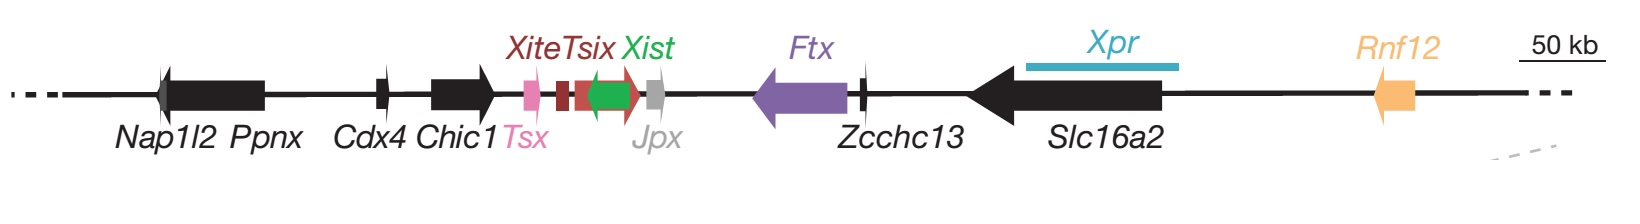
\includegraphics[scale=0.3]{geneSequencesTADDandE}
\caption{\scriptsize{The genes and non protein coding regions of TAD D and E. Image taken from from Nora et al.Nature. 2012 Apr 11;485(7398):381-5 \cite{nora2012spatial}}}
\label{genesOfTadDandE}
\end{figure}

\subsection{A short review of the 5C method}
The 5C method \cite{dostie2006chromosome} relies on the first steps of the seminal 3C method proposed by \href{http://www.sciencemag.org/content/295/5558/1306.full.pdf}{Dekker et al. 2002} \cite{dekker2002capturing}. 
From the supplementary material of the article by \href{http://www.sciencemag.org/content/295/5558/1306/suppl/DC1}{Dekker et al}. The steps of the 3C can be described as follows (see also Figure \ref{3Cschematic}):

\begin{enumerate}
\item Roughly $10^8$ intact nuclei are isolated
\item Nuclei are \href{http://en.wikipedia.org/wiki/Crosslinking_of_DNA}{cross-linked} by using $1\%$
\href{http://en.wikipedia.org/wiki/Formaldehyde}{formaldehyde} or its relative paraformaldehyde for 10 minutes, which induces protein-protein and DNA-protein cross-linking. The cross-link is made by formaldehyde in the guanine nucleotide, between DNA-bound proteins and the nucleotide. 
\item All non cross-linked proteins are removed.  It is important to note that the DNA is purified only After the cross-links were made.
\item A site-specific restriction enzyme (ECOr or HindIII, 6bp cuter) is used to digest the cross-linked DNA for 1 hour. 
\item The restriction enzymes are inactivated using SDS and incubation for 20 minutes.
\item The reaction is 15 times diluted to favor relevant DNA end ligation.
\item The free ends of the cleaved DNA are ligated (DNA is still cross-linked with proteins) for 45 minutes using ligase.
\item Reverse cross-linking by overnight incubation: the cross-links are destroyed, leaving segments of ligated DNA. The reverse cross-linking is done by incubation at $70^0$.
\item DNA is purified from non cross-linked proteins.
\item The products of the ligation are detected and quantified using PCR. 
\item a control template is created by using the same restriction enzyme on non cross-linked DNA and ligation of DNA fragments without dilution
\end{enumerate}

\begin{figure}[H]
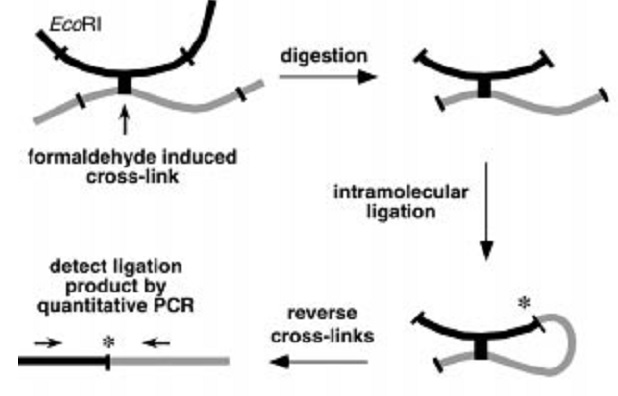
\includegraphics[scale = 0.4]{3Cschematic}
\caption{\scriptsize{A schematic representation of the 3C method. Image taken from \href{http://www.sciencemag.org/content/295/5558/1306.full.pdf}{Dekker et al. 2002}\cite{dekker2002capturing}}}
\label{3Cschematic}
\end{figure}

\section{The Experimental Data}
Two replicates of 5C experiments were conducted taking into account the Xic region. The data was coarse-grained as explained in \ref{coarseGrainingOfEncounterData}.
The encounter data includes the number of encounters between 14,508 genomic segments. Each genomic segments is defined by the start and end bead.

\subsection{Coarse-graining of the data}\label{coarseGrainingOfEncounterData}
The following paragraphs are an adapted version of the text in from Giorgetti et al. \cite{giorgetti2014predictive} supplementary material.

In the genomic region of the TAD D and E, 124 forward (FOR) and 126 reverse (REV) primers anneal to alternate HindIII restriction fragments of variable size. 
Since the average length of FOR and REV fragments in this region is 3078 bp, a 3000-bp beads was chosen, resulting in polymers of N=108 beads in the case of TAD D alone (chrX:100378306-100699670, total length 321’364 bp) and $N=307$ beads in the case of TAD D+E (total length 92’0432 bp). Thirty five percent of restriction fragments are longer then 3000 bp and will be mapped on multiple beads, while the remaining $65\%$ will contribute together with their nearest neighbor to define the expected contacts of single beads.

To simulate 5C experiments, the uneven sampling of the genomic region provided by restriction fragments of different length must be mapped onto the even sampling provided by equally spaced beads. This is performed as follows:

\begin{enumerate}
\item The $5$ end of the first bead in the chain is positioned at the 5’ end of the first restriction fragment in the region of interest 
\item Each restriction fragment in the region is assigned two indices $i$ and $j$ $(i,j=1…N)$ corresponding to the beads to which its 5’ and 3’ ends overlap.
\item 5C counts corresponding to each pair of restriction fragments are assigned to the corresponding pairs of indices (i,j) and (h,k), for example:
\item If two or more consecutive FOR or REV restriction fragments map to the same bead, their contributions are summed ($<10\%$ of all interactions).
\item 5C counts of two experimental replicates are averaged for each pair of restriction fragments and their standard deviation is taken as a measure of experimental uncertainty.
\end{enumerate}

\subsection{The encounter matrix}
The data provided by Giorgetti et al.\cite{giorgetti2014predictive} contains the encounter frequency of beads (not segments!) constructed as explained in \ref{coarseGrainingOfEncounterData}. Sorting the encounter data into a 2D matrix results in a 307 by 307 array. Reminder: beads are numbered sequentially from the 5-end to the 3-end of the polymer.

\section{Analysis of the data}

\subsection{From encounter frequency to encounter probability}
We start by transforming the encounter data into encounter probability. Each line of the encounter matrix is divided by the sum of all encounters of the line.

\subsection{Showing the TADs}
TADs are seen by displaying the normalized encounter data, after removing closest beads data from the matrix of encounters. 
The normalization is done by taking each row $k$ of the encounter matrix, removing the data for the closest neighbors of bead $k$ and dividing by the sum of the row. A median filter of size 30 beads is then applied to the image (see methods in \cite{nora2012spatial}). 
 
\subsection{Symmetry of encounter frequency data}
We next examined whether the data can be regarded as symmetric in the sense of encounter probabilities for each bead. That is, whether bead $k$ has the same probability to meet its closest neighbors from the right and left in the linear chain, or not.  

The symmetry of encounter frequency data is shown by measuring the left and right encounter frequencies of each one of the beads comprising the chain.
The left and right encounter data are defined in terms of bead index, where for the bead $j$ the left encounter frequencies are defined as a vector of length $j-1$ with the encounter data of bead $j$ with $1,..,j-1$, and $j+1,..,N$ for the right encounter frequencies. 

For bead index $j=1,...,N$ we have different number of beads on the left and right. For comparison, we need to match the number of beads from the left and right for each bead. The number of beads on the left and right of bead $j$ is then taken to be $n_j=min(j-1,N-j+1)$. 
Let $L_j$ be the left encounter data, $R_j$ be the right encounter data vectors of lengths $n_j$
\begin{equation*}
L_j=\left[e(j-1),e(j-2),...e(j-n_j)\right] 
\end{equation*}
and 
\begin{equation*}
R_j=\left[e(j+1), e(j+2),...,e(j+n_j)\right]
\end{equation*}
where $e(k)$ is the encounter frequency of the $k^{th}$ closest bead to the bead $j$. Note the reverse order of $L_j$.

We normalize each vector by dividing it by the sum of its encounters
\begin{equation*}
\hat{L_j} =\left[e(j-1),e(j-2),...,e(j-n_j)\right]/\sum_{k=j-n_j}^{j-1}e(k)
\end{equation*}
and similarly for $\hat{R}_j$.

To test the difference between left and right frequencies, we calculate the mean difference by 
\begin{equation*}
d_j=\frac{1}{n_j}\sum_{k=1}^{n_j} \left(\hat{L_j}(k)-\hat{R_j}(k)\right)
\end{equation*}

The Figure \ref{resultsOfFrequencyDifference} below shows the results of plotting the mean difference for the two replicates of the 5C data 

\begin{figure}[H]
\includegraphics*[scale=0.3]{symmetryOfEncountersRep1.jpg}
\includegraphics*[scale=0.3]{symmetryOfEncountersRep2}
\includegraphics*[scale=0.3]{symmetryOfEncountersAverage}
\caption{\scriptsize{ The mean difference (y axes) between left and right encounter frequencies for each bead number (x axes) is shown for Rep1 (top left) Rep2 (top right) and average (bottom)}}
\label{resultsOfFrequencyDifference}
\end{figure}  

The red lines in the Figure \ref{resultsOfFrequencyDifference} signify the mean of the difference data. For the three figures it is of the order $10^{-18}$. When points are missing, it means that the segment (restriction segment) occupies more than one bead, therefore the encounter data is zero there. 

We can therefore treat the right and left data in the same manner and 'fold' the encounter data such that from now on we test the encounter data by bead distance. the 'folded' encounter data will be called just the encounter data from now on. 

\subsection{Peaks of the encounter data}
For some beads the encounter data shows peaks at some distance from the origin. 
These peaks represent a frequent encounter with a distal part of the chain. The list of bead numbers and the frequent encounter they have with the distal chain parts (represented by bead numbers) is summarized in Table \ref{nonNeighborBeadEncounterTable}
% old table (One Sided)
\begin{table}[H]\label{nonNeighborBeadEncounterTable}
\begin{tabular}{l l l}
bead numbers & encountered beads & TAD\\
\hline
23-26   & 280-290 & $D\leftrightarrow E$\\
49-53   & 148-155 & $D\leftrightarrow E$\\
56-59   & 80-90   & $D\leftrightarrow D$\\
115-117 & 165-170 & $E\leftrightarrow E$\\
161-162 & 187 190 & $E\leftrightarrow E$\\
182-184 & 260-264 & $E\leftrightarrow E$\\
185-186 & 253-255 & $E\leftrightarrow E$\\
234-236 & 184-189 & $E\leftrightarrow E$\\
234-236 & 4-11    & $E\leftrightarrow D$\\
243     & 88      & $E\leftrightarrow D$\\
264     & 89-90   & $E\leftrightarrow D$\\
274-277 & 113-120 & $E\leftrightarrow D(?)$
\end{tabular}
\end{table}

% new Table (two sided)
\begin{table}[H]
\begin{tabular}{l l l l}
bead numbers & encountered beads & TAD & rep\\
\hline
1       & 86      & $D\leftrightarrow D$& 1 \\
6       & 81      & $D\leftrightarrow D$& 1 \\
6       & 227-229 & $D\leftrightarrow E$& 1 \\
6       & 243     & $D\leftrightarrow E$& 1 \\
7       & 81      & $D\leftrightarrow D$& 1 \\
7       & 226-229 & $D\leftrightarrow E$& 1 \\
7       & 247     & $D\leftrightarrow E$& 1 \\
10      & 77      & $D\leftrightarrow D$& 1 \\
10      & 77      & $D\leftrightarrow D$& 1 \\
23      & 293     & $D\leftrightarrow E$& 1 \\
24      & 264     & $D\leftrightarrow E$& 1 \\
25      & 285     & $D\leftrightarrow E$& 1 \\
26      & 285     & $D\leftrightarrow E$& 1 \\
26      & 86      & $D\leftrightarrow D$& 1 \\
26      & 59-74   & $D\leftrightarrow D$& 1 \\
49-53   & 150     & $D\leftrightarrow E$& 1 \\
64-66   & 287     & $D\leftrightarrow E$& 1 \\
65-66   & 34      & $D\leftrightarrow D$& 1 \\ 
64,67-69& 26      & $D\leftrightarrow D$& 1 \\       
71      & 24      & $D\leftrightarrow D$& 1 \\
72-75   & 26      & $D\leftrightarrow D$& 1 \\

\end{tabular}
\end{table}

The question arises as to whether these frequent encounter represent a loop in the polymer chain or is it the results of the 3D structure of the folded polymer? Since the 5C data is essentially taken over millions of cells it remains to show that these encounters (or loops) are indeed conserved elements of the Xic region.

\subsection{Fitting the encounter data}
In this and subsequent sections we work with the first replicate of the data.

To examine the behavior of the polymer as a whole, we fit for each bead's encounter data 
(row or column) a function of the form 
\begin{equation}\label{fitModel}
\log(e_j(t))= \log(At^{-B})= \log(A)-B\log(t)
\end{equation}
where $t$ represents the distance in bead units to bead $j$, and $e_j(t)$ is the normalized encounter data by distance for bead $j$, $A$ and $B$ are parameters to be determined by the fitting process. 

\begin{figure}[H]
\includegraphics*[scale=0.2]{EncounterFrequenciesByDistanceRep1}
\caption{\scriptsize{The encounter probability of each bead (Y axis) as a function of bead distance (X axis). The dashed red rectangles shows places of prominent non-nearest neighbors encounters}}
\end{figure}

The fitted exponent ($B$) and bias ($A$) values obtained by minimizing the error in the model \ref{fitModel} are shown in Figure \ref{fittedExpAndBias}
\begin{figure}[H]
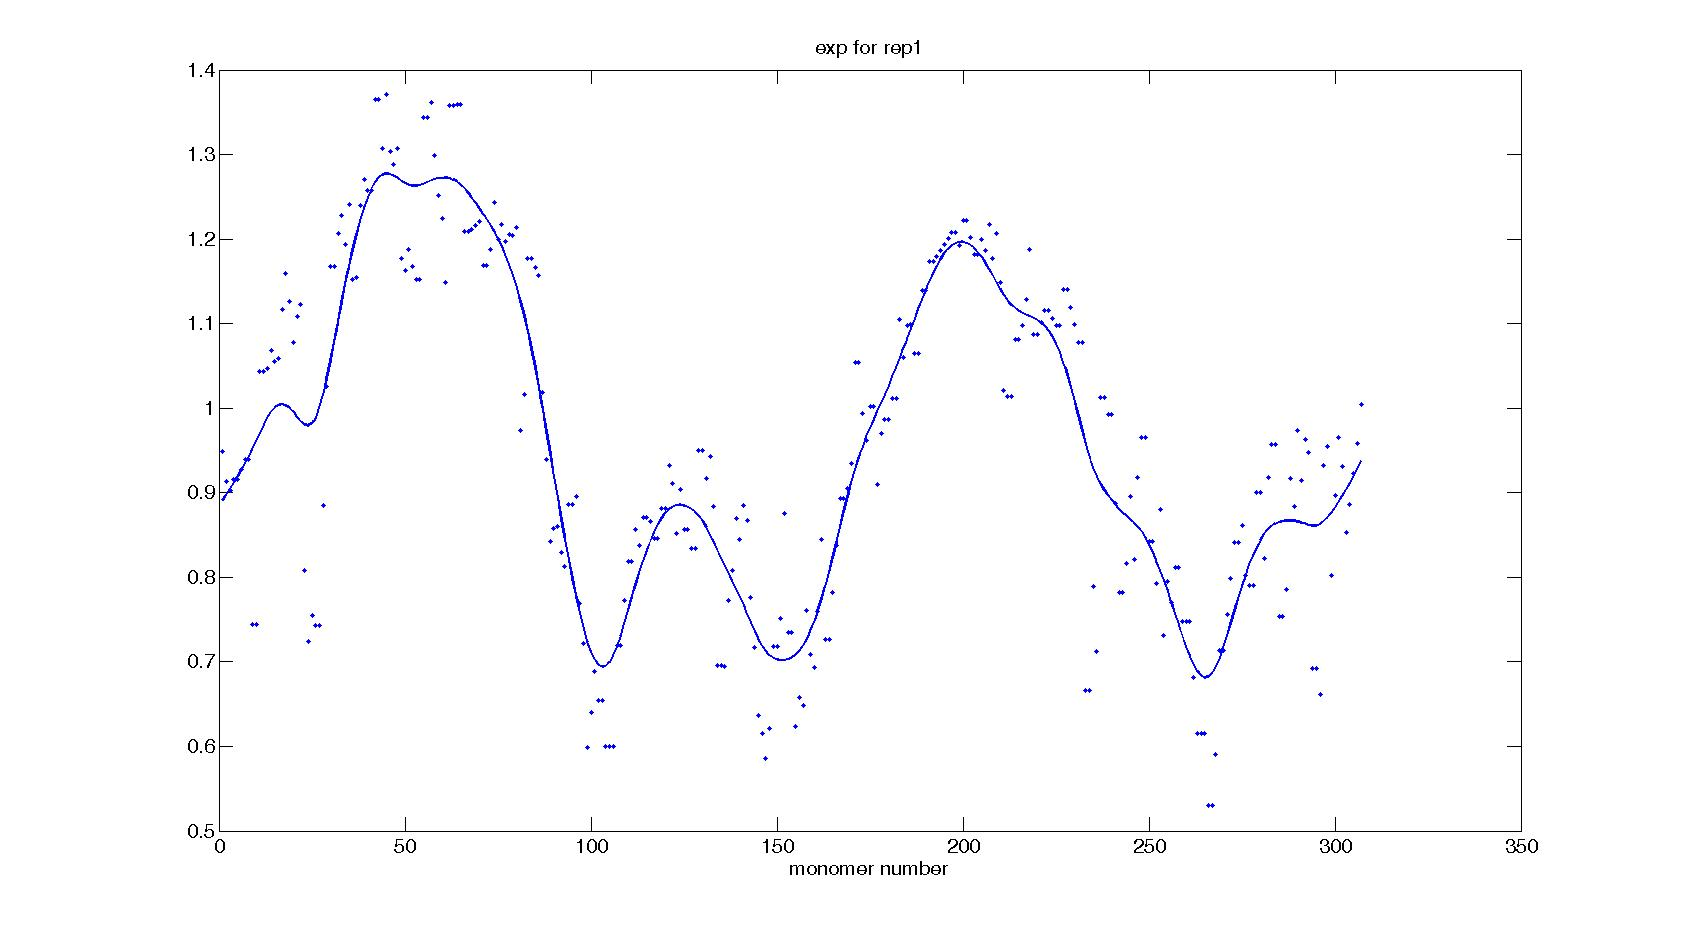
\includegraphics[scale=0.15]{fittedExpValuesWithSplineRep1}
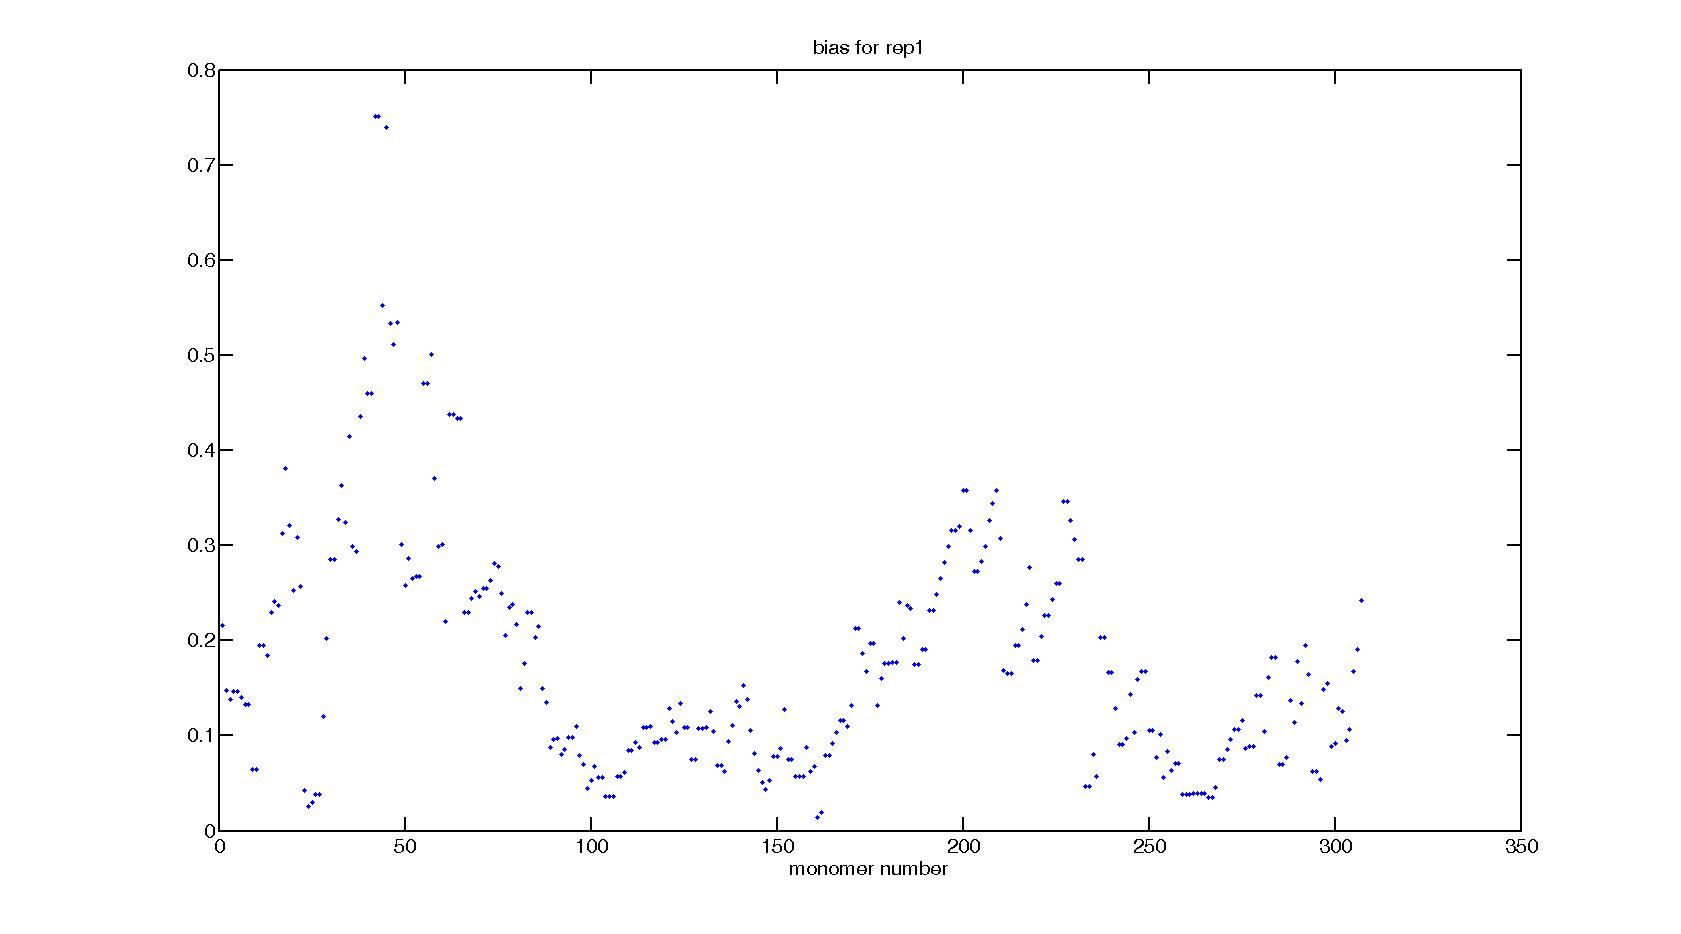
\includegraphics[scale=0.15]{fittedBiasValuesRep1}
\caption{\scriptsize{The fitted exponent (top) and bias (bottom) for each bead index. In the upper plot, the continuous curve represents a smoothing of the fitted exponent values using a smoothing spline with tolerance of 2 (see Matlab documentation on \href{http://www.mathworks.fr/fr/help/curvefit/spaps.html}{spaps} function)}}
\label{fittedExpAndBias}
\end{figure}

%TODO: remove the following paragraph
It is apparent from Figures \ref{fittedExpAndBias} that there is some correlation between the fitted exponent values and the bias (indeed, since the integral of each function should be 1). To see it more clearly, we plot the fitted exponent and bias values on the same axes (Figure \ref{fittedExpVsFittedBias}). 

\begin{figure}[H]
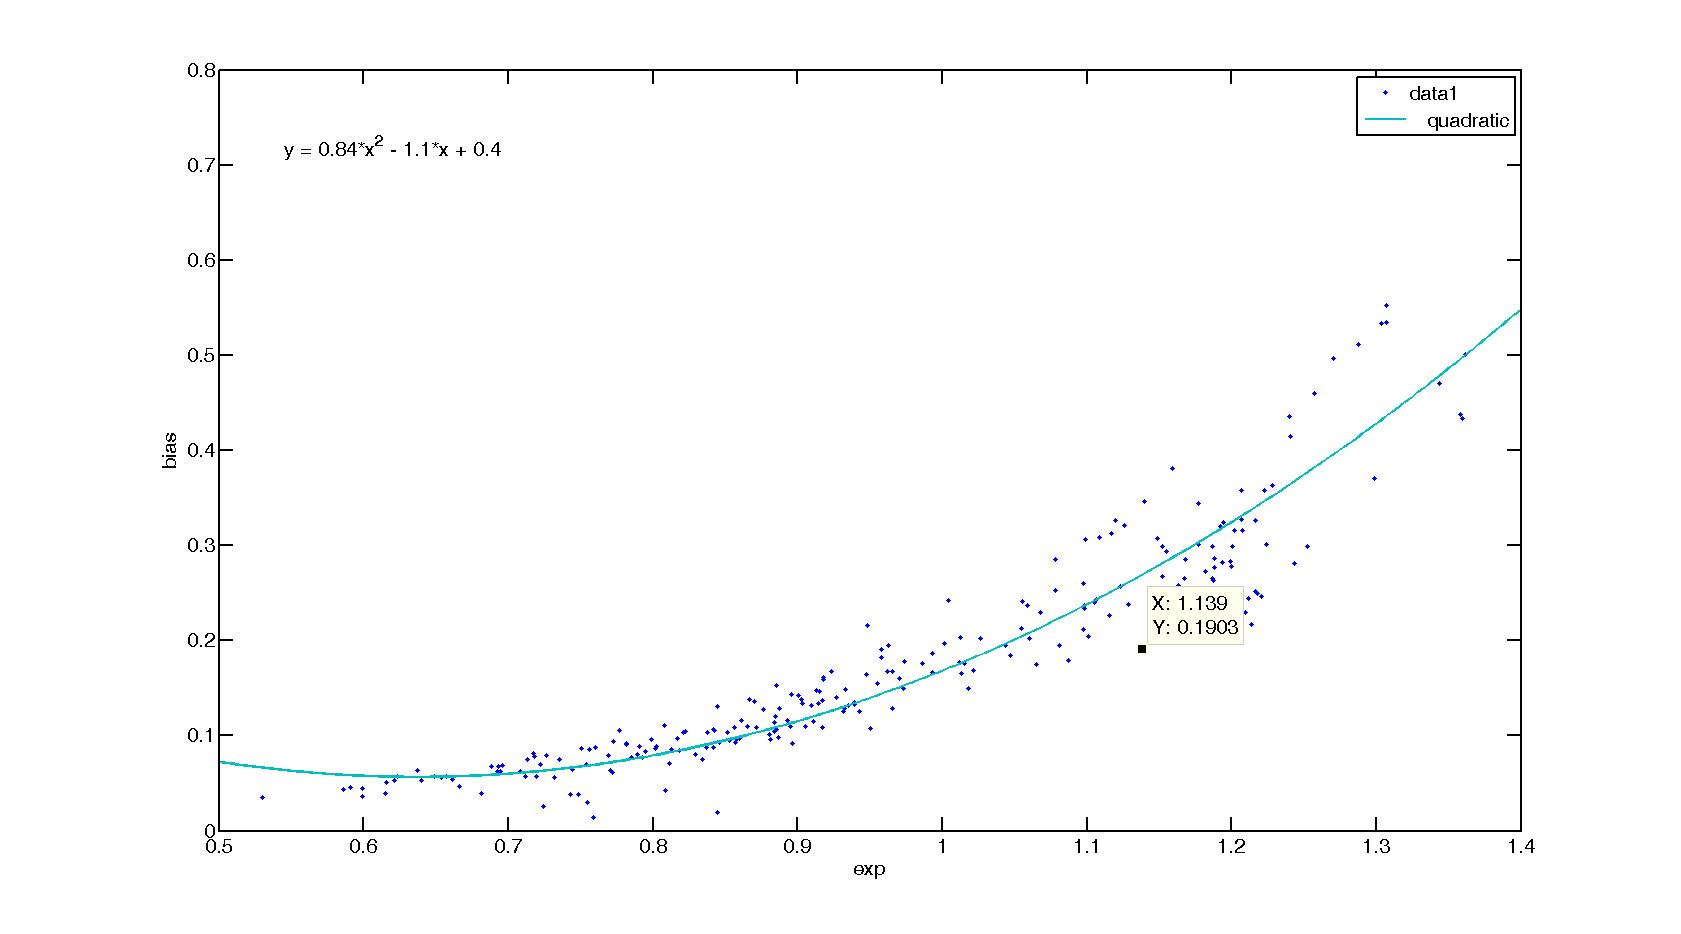
\includegraphics[scale=0.15]{fittedExpVsFittedBias}
\caption{\scriptsize{The fitted bias values are plotted as a function of fitted exponent values. The continuous cyan curve is a quadratic fit to the data. The equation that represents the fit appears in the top left corner}}
\label{fittedExpVsFittedBias}
\end{figure}

In Figure \ref{fittedExpAndBias} top box, we see that the fitted exponent curve is somewhat tri-modal. With one peak located in roughly at bead 54, one at 125, and the left most at 200. The first and the last places correspond the mid points of the two TADs of the encounter. 

From Figure \ref{fittedExpVsFittedBias} we see that the bias values tend to increase positively with the exponent. A quadratic curve was fitted to the fitted exponent vs. fitted bias data and resulted in values
\begin{equation}\label{fitModelForExpVsBiasData}
B^* = 0.84A^2-1.1A+0.4
\end{equation}

 An important issue to address no is what is the validity of the fitted values?
Comparing the actual bias values to the prediction of the fitted quadratic curve \ref{fitModelForExpVsBiasData} we get the difference curve as appears in Figure \ref{diffFittedBiasVsModelBias}. The mean difference between model predictions and model fit is 0.0274. We see that for the beads 35-50 there is a disagreement between prediction of model \ref{fitModelForExpVsBiasData} and model \ref{fitModel} (green dashed box in Figure \ref{diffFittedBiasVsModelBias}). 

We therefore conclude that further in-depth evaluation of parameters is needed in specific regions of the polymer ot gain insight into the nature of the departure from the 'average' model fitted.

\begin{figure}[H]
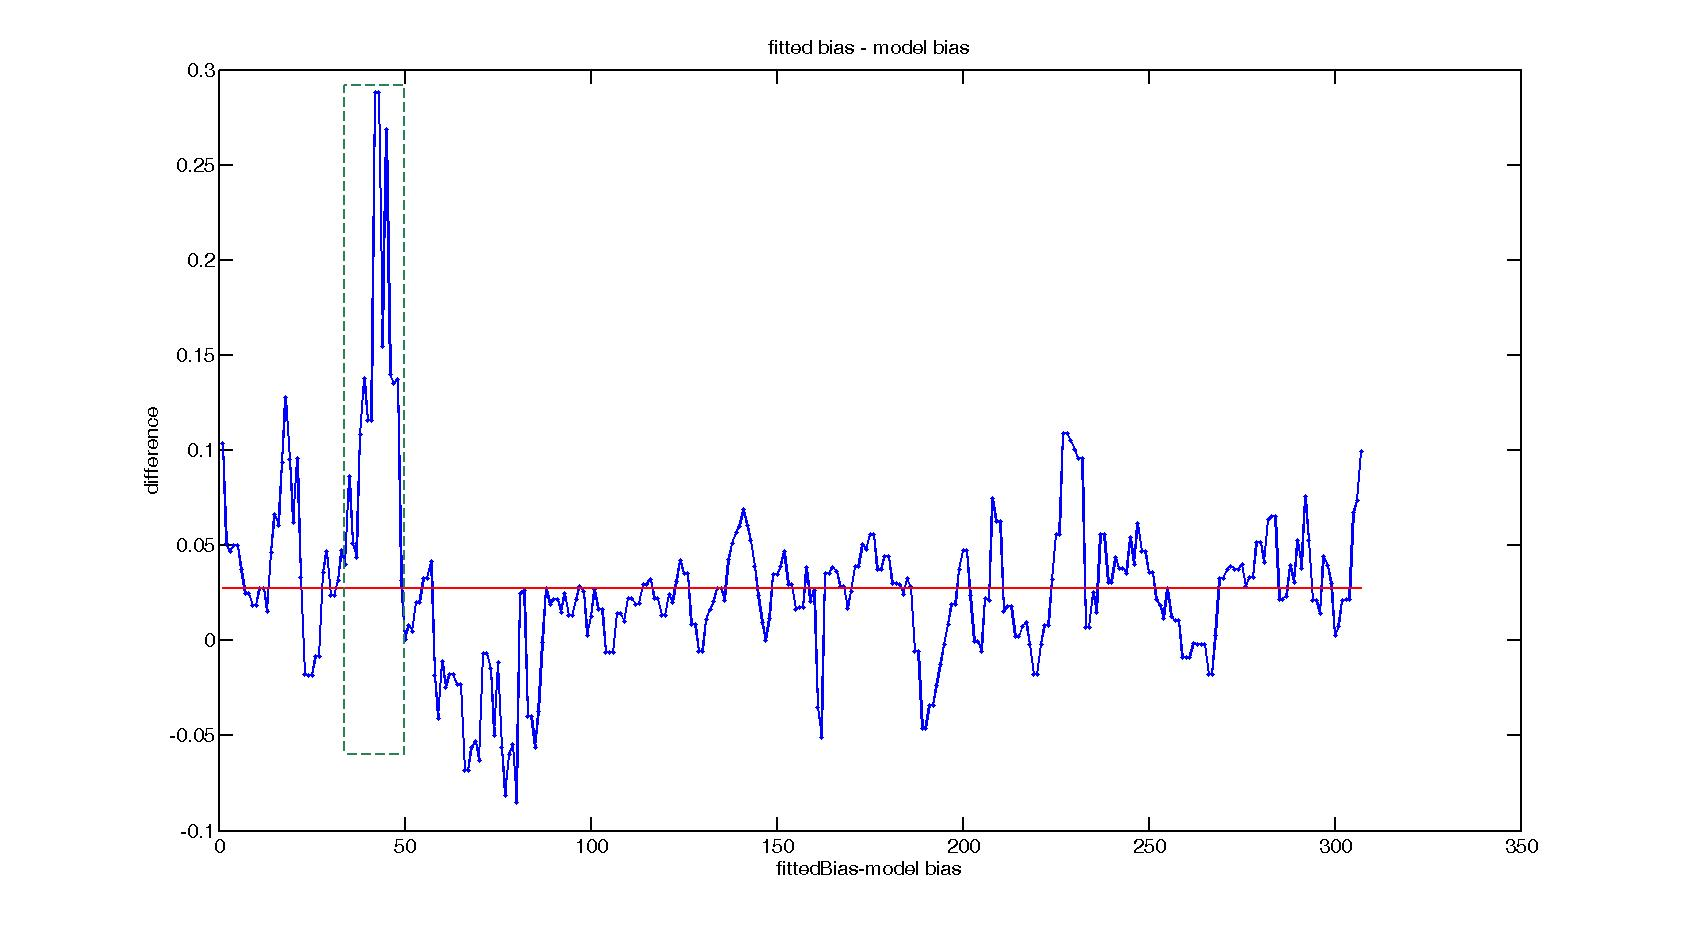
\includegraphics[scale=0.15]{diffFittedBiasVsModelBias}
\caption{\scriptsize{The difference between the fitted bias values $B$ and the values predicted by model \ref{fitModelForExpVsBiasData}. The red line shows the mean of the difference and equals 0.0274. The green dashed rectangle shows the beads for which the model prediction and the data fitting do not agree. It corresponds to roughly the beads 35-50}}
\label{diffFittedBiasVsModelBias}
\end{figure}

\subsection{Heterogeneity of the parameters over the beads}
The question arises as to whether the beads behave in a similar manner in terms of parameter values (i.e obey the same model rules), and if not, would it be possible, just by assuming a model, to identify beads belonging to the same group, and elucidate the similarity or difference between groups of beads. 
We start by looking at adjacent beads properties according to the resulting parameter fitted.
To simultaneously see the heterogeneity of the fitted parameters over all beads, we calculate the pairwise difference between parameters of the beads. 
the resulting matrices take the shape

\begin{figure}[H]
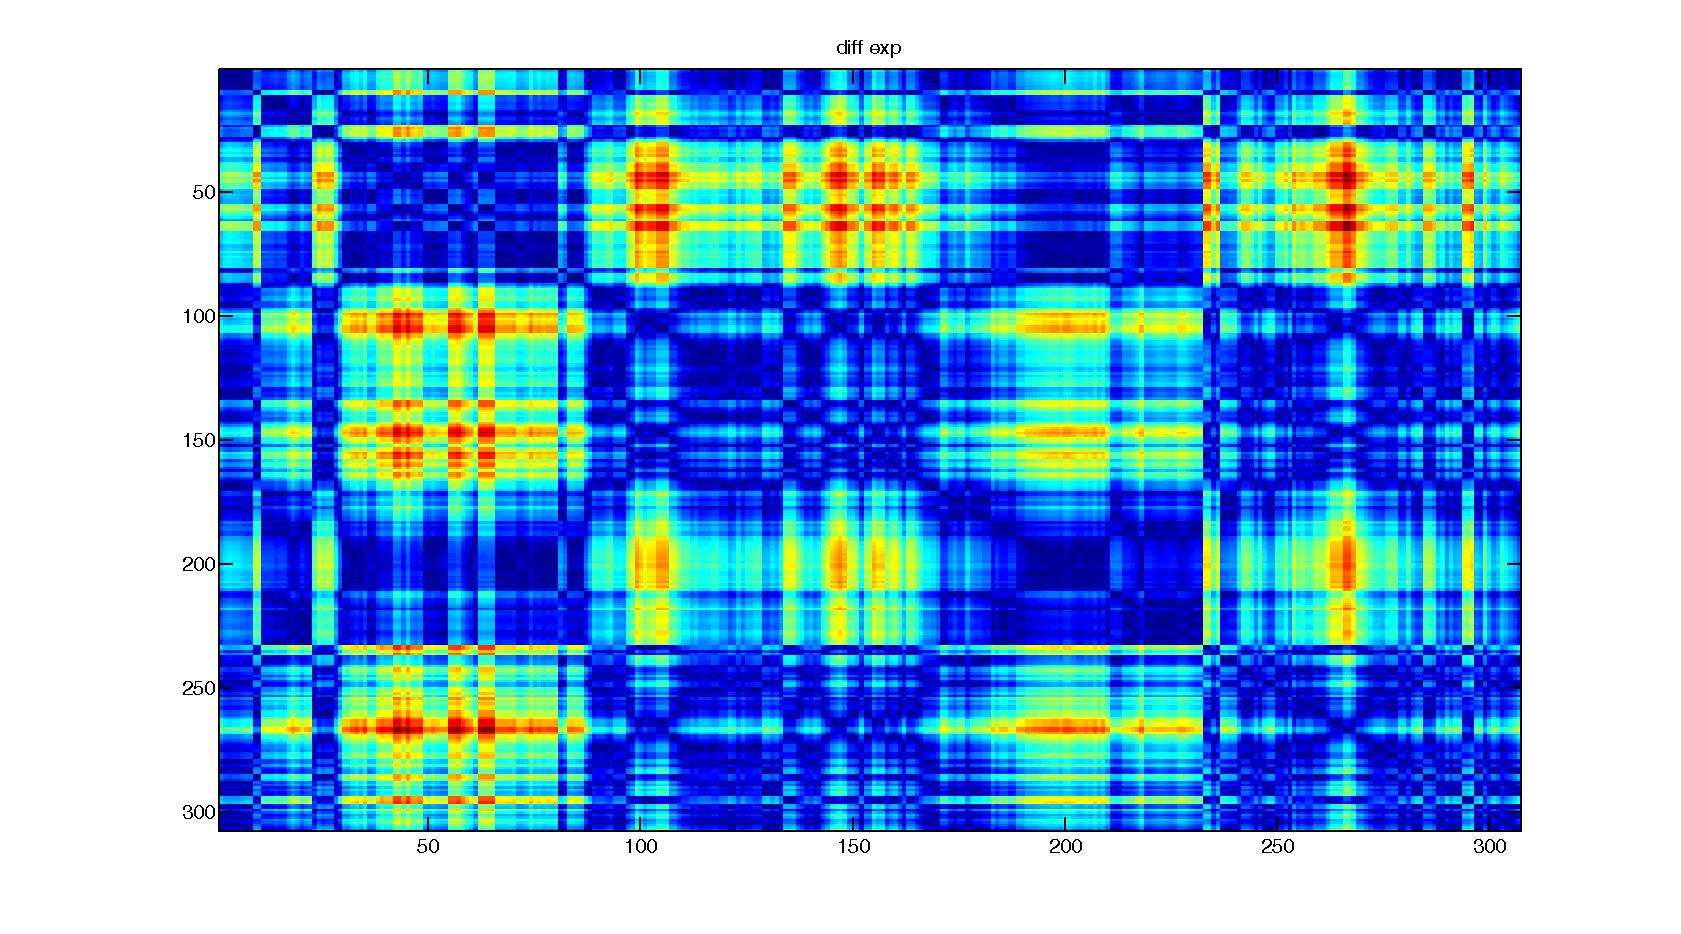
\includegraphics[scale=0.15]{diffFittedExpRep1}
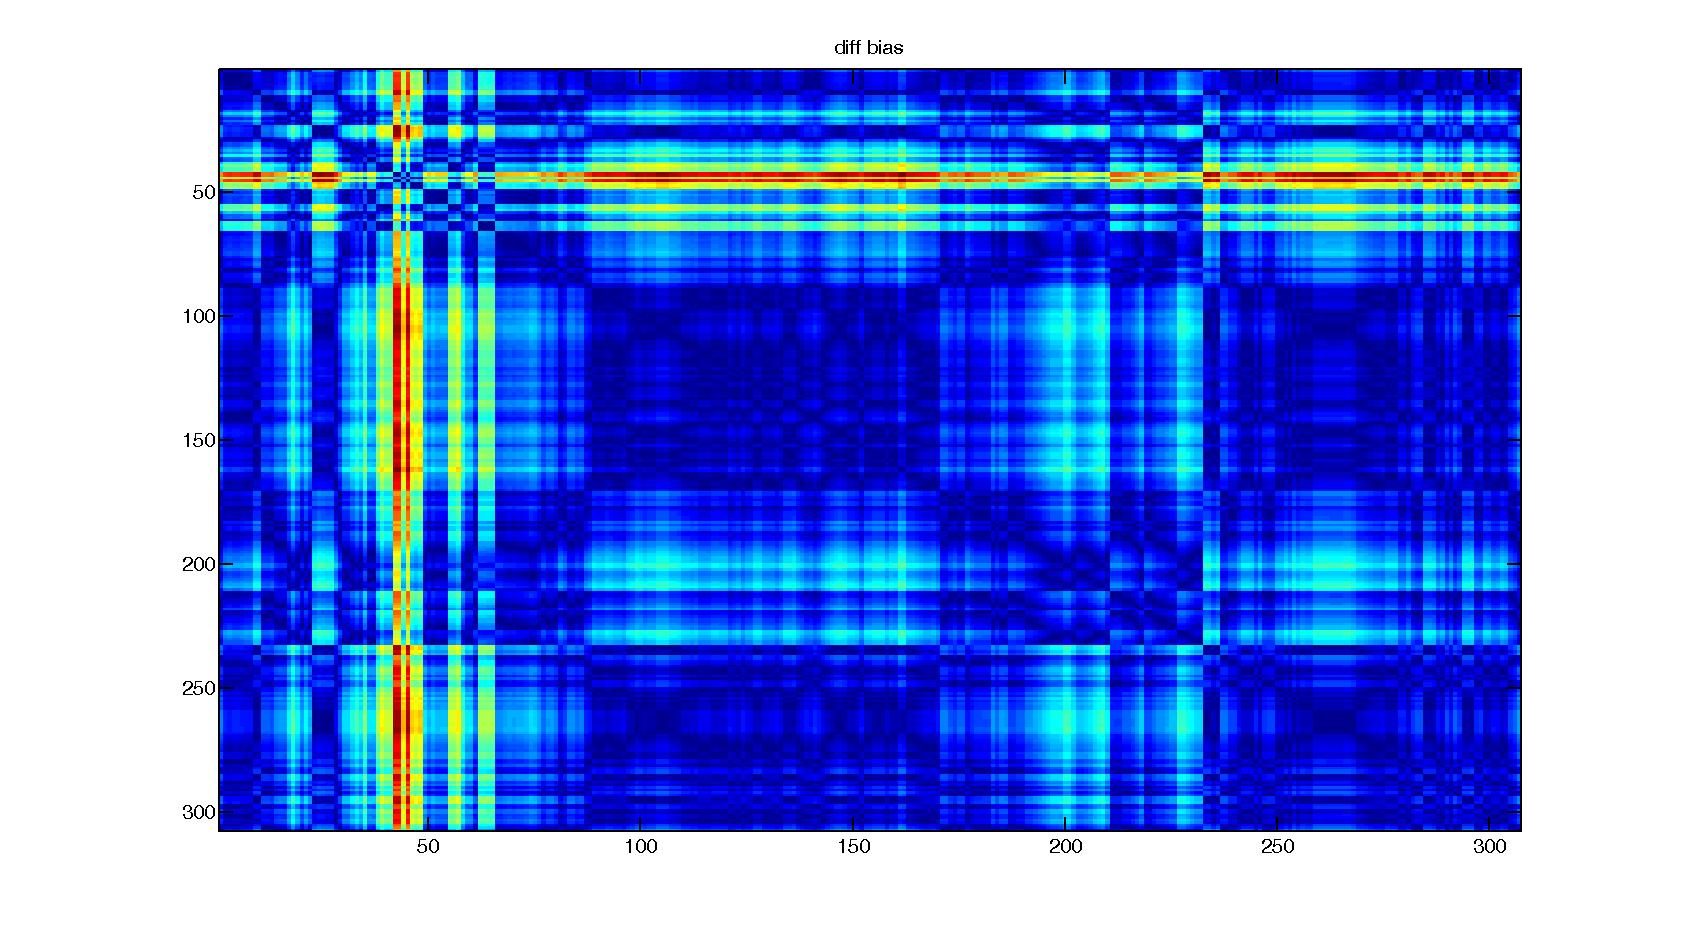
\includegraphics[scale=0.15]{diffFittedBiasRep1}
\includegraphics[scale=0.15]{normDiffFittedExpfittedBiasRep1}
\caption{\scriptsize{The norm of the difference between the fitted parameters from model \ref{fitModel} in a pairwise manner. the columns and rows represent bead numbers. The pairwise exponent difference norm (top), the pairwise difference norm for bias (middle); the norm of the two difference matrices (bottom)}}
\label{diffFittedParametersRep1}
\end{figure}

It is now also apparent from Figure \ref{diffFittedParametersRep1} that beads 35-50 have different bias values then expected. To find beads for which the exponent values agree but the bias values do not, we search for a threshold for the difference of exponents and bias below which it could be said that values are similar. 
For this end, we can consider the data as having 'low' and 'high' difference values. 
We search for a values $v_{exp}$ and $v_{bias}$ for which the 'within' group variance is low and the 'between' group variance is the highest. 
Such approach leads naturally to employ the \href{http://en.wikipedia.org/wiki/Otsu's_method}{Otsu} method. Using this method on the matrix, the value of $v_{exp},v_{bias}$ are found to be 

\begin{equation}
v_{exp}= 0.262
\end{equation}
\begin{equation}
v_{bias}=0.18
\end{equation}

\section{Simulations}
\subsection{Initial settings}
For the subsequent simulations, unless stated differently, we determine the simulation time step,$\Delta t$ and the simulation time as follows. 
the simulation step $\Delta t$  was determined such that it will prevent simulation 'blow-ups'
\begin{equation*}
 \Delta t = \frac{b^2}{12D}
\end{equation*}
Which is the values that stabilizes the numerical solution to the ode with no noise. when noise is present, this values can be increased.

The chain relaxation time is given by 
\begin{equation*}
\tau_p = \frac{b^2\Delta t}{12d^2\sin^2(\frac{p\pi}{2N})}
\end{equation*}
where $p$ is the mode number. For simulations we use the relaxation time of the slowest mode $p=1$.

\subsection{Verification of the validity of the output of the simulation framework}
Here we make sure that the output simulation framework obeys the expected behavior of the Rouse polymer. 
A polymer of 64 beads, with no cross-linking is simulated for $40,000$ steps, the STD of link length was set to $b=0.1$. The result is presented in Figure \ref{distanceMatrix64Beads}

\begin{figure}[H]
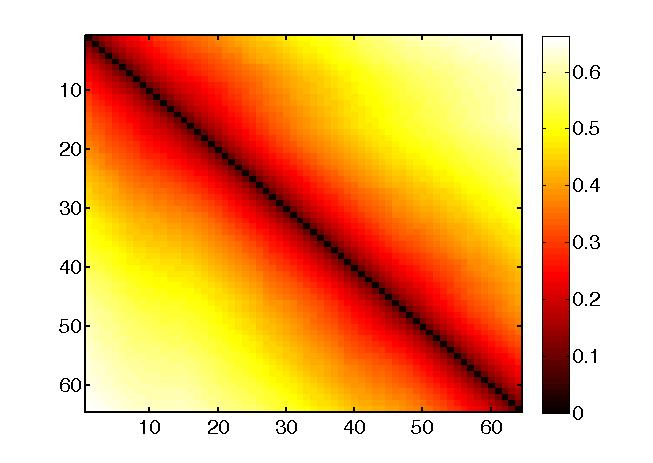
\includegraphics[scale=0.3]{distanceMatrix64Beads}
\caption{\scriptsize{The mean bead distance matrix after $50,000$ steps of the Rouse model}}
\label{distanceMatrix64Beads}
\end{figure}

For an easier comparison of the simulation output with theoretical results, we work from now on with the Root-Mean-Square (RMS) distance between beads. 

To see the expected increase in distance, we plot the cross-section of the RMS distance of the first bead to beads $2,3,..,64$. The distribution of distances between any two beads $n$ and $m$ of the Rouse polymer, have the following distribution
\begin{equation}
\Phi(R_n-R_m,n-m)=\left[\frac{3}{2\pi b^2|n-m|} \right]^{3/2}\exp{\left[-\frac{3(R_n-R_m)^2}{2|n-m|b^2} \right]}
\end{equation}
Where, $R_n$ is the vector of coordinates of bead $n$. The equation above is the consequence of the fact that the sum of normally distributed random variables is again a normally distributed random variable. In addition, it can be shown that 
\begin{equation}\label{RmsDistance}
<(R_n-R_m)^2>=|n-m|b^2
\end{equation}
Using the result above we compare the RMS distance between bead $1$ and beads $2,3,..,64$ with the function $|n-m|b^2$, appearing in equation \ref{RmsDistance}, with $b=0.1$. As can be seen from Figure \ref{rmsDistanceBead1ToBeads2To64AndTheoreticalResults}, there is an excellent agreement between the output of the simulations and the theoretical results.

\begin{figure}[H]
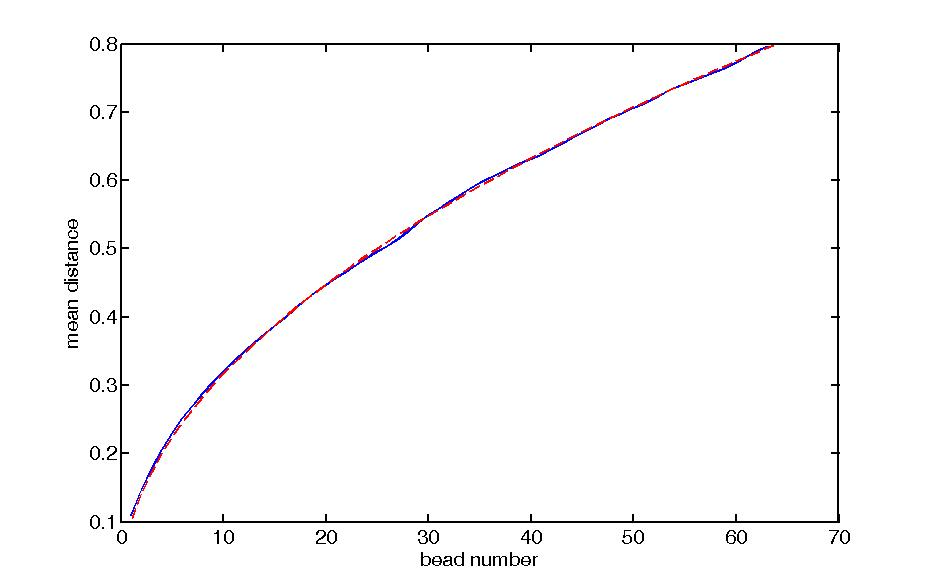
\includegraphics[scale=0.3]{rmsDistanceBead1ToBeads2To64AndTheoreticalResults}
\caption{\scriptsize{The RMS distance of bead 1 to all other 63 beads is plotted (blue curve) vs. the theoretical result (dashed red curve) $dist(1,n)=nb^2$. As can be seen, there is an excellent agreement between the curves, indicating that the simulation framework operates as expected}}
\label{rmsDistanceBead1ToBeads2To64AndTheoreticalResults}
\end{figure}

The RMS distance between adjacent bead was found to be 0.105, in agreement with  the bond length $b=0.1$. The mean square end-to-end distance was found to be 0.6319, in agreement with the expected 0.64. Overall we can conclude that the system operates as expected.

\subsubsection{The encounter frequency}
According to the theory, the encounter frequency of a bead $m$ in a Rouse chain as a function of the distance of beads from it on the linear chain, should be proportional to $1/|m-n|$, where $n\ne m$ is the distance in bead units. To see that the simulation framework obeys this rule, the encounter frequency matrix was calculated. The encounter distance was set to $0.1$, the matrix is presented in Figure \ref{encounterMatrix64Beads}. To see the decay of the encounter matrix, we  plot the normalized encounter events of bead 1, and present the fit of the function
\begin{equation}
y = ax^{-b}
\end{equation}
The encounter data was normalized prior to fitting by dividing it by the sum of encounter of bead 1. The parameters fitted were found to be $a=0.2436$ and $b=1.036$, in agreement with the expected $e(1)\propto 1/n$

\begin{figure}[H]
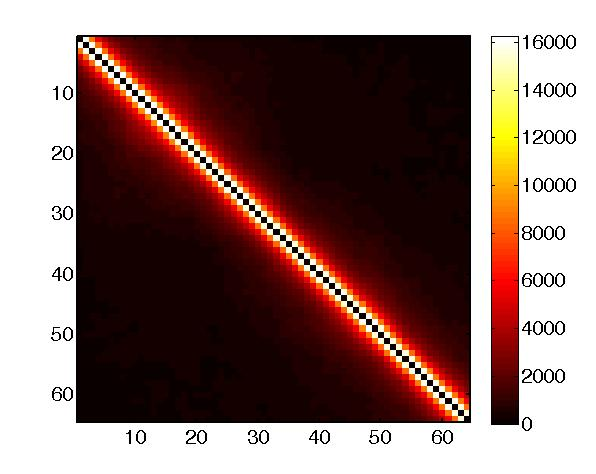
\includegraphics[scale=0.3]{encounterMatrix64Beads}
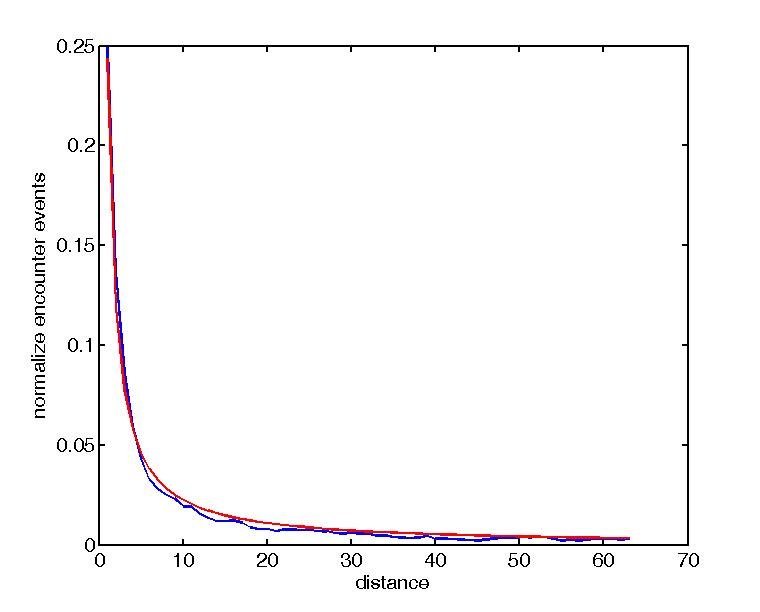
\includegraphics[scale=0.3]{encounterFrequencyBead1WithFit}
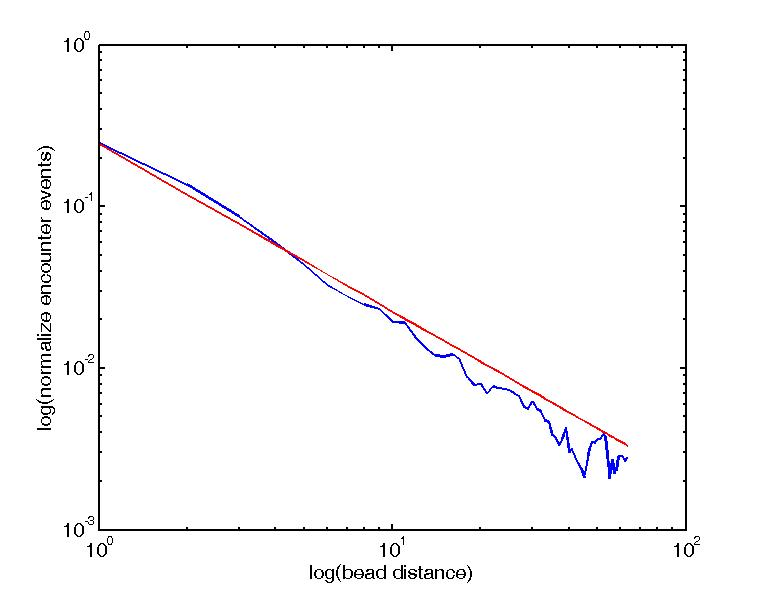
\includegraphics[scale=0.3]{encounterFrequencyBead1WithFitLogScale}
\caption{\scriptsize{The encounter frequency and verification of theoretical results. The encounter matrix (top left) for a 64 beads Rouse chain. The decay of the rows of the encounter matrix is presented for the first bead (top right) for which we have the most number of beads (blue line) and a fit to the encounter curve (red line). the encounter frequency of bead 1 in a log-log scale (bottom left, blue curve) and a fit according to the theory (red line).}}
\label{encounterMatrix64Beads}
\end{figure}

\subsection{Simulating cross-linked polymer with a single link}
Next, we test the behavior of the distance matrix for a 64 bead polymer for which bead 24 and 44 are cross-linked, creating a loop of size 20 beads. 
The simulation is run from relaxation time, a total of $50,000$ steps. The relaxation time is determined according to the formula
\begin{equation}
\tau_p = \frac{b^2\Delta t}{12d^2\sin^2(\frac{p\pi}{2N})}
\end{equation}
For  $\Delta t=10^{-4}$, $p=1$, $d=\sqrt{2D\Delta t}$, $N = 64$, we get 
\begin{equation}
\tau_1 = 57.68 
\end{equation}
minutes, which is the relaxation time of the first Rouse mode derived from the cross-correlation function. 

\begin{figure}[H]
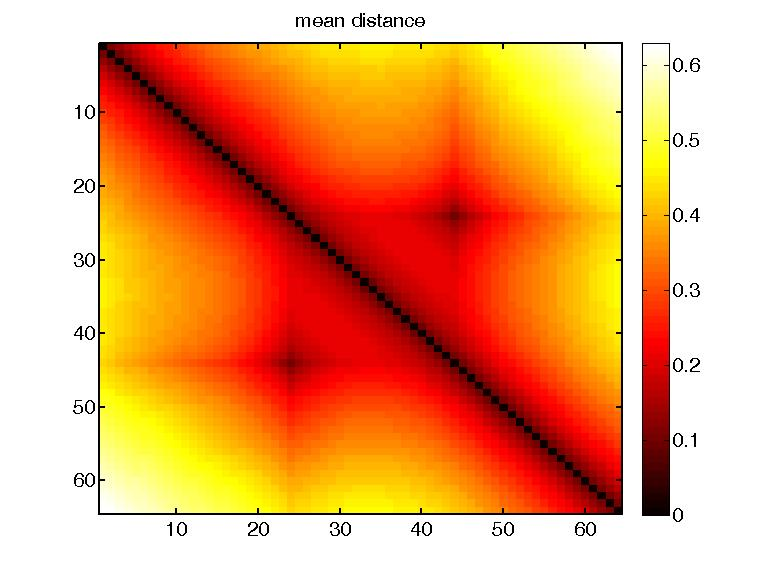
\includegraphics[scale=0.3]{distanceMatrix64BeadsConnect24And44}
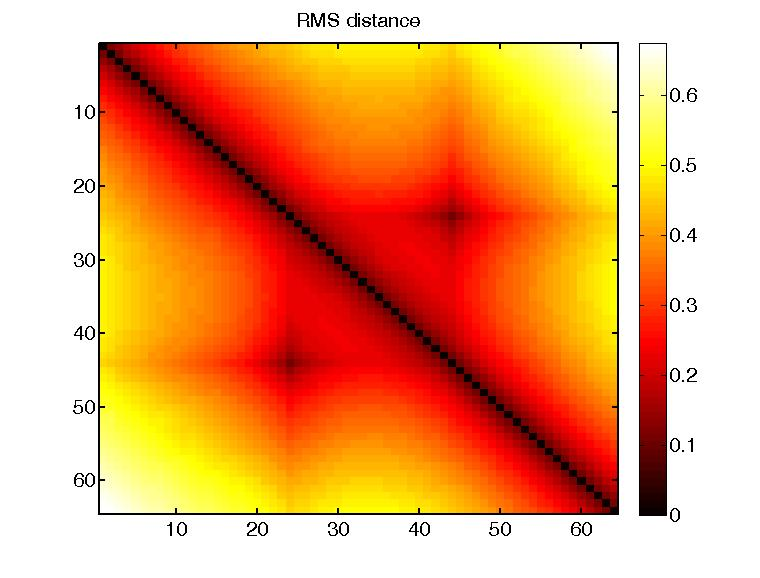
\includegraphics[scale=0.3]{rmsMatrix64BeadsConnect24And44}
\caption{\scriptsize{mean Distance matrix (left) and RMS distance matrix (right) over 50,000 steps of the simulation. Beads 24 and 44 are connected in a polymer of length 64 beads. As expected,the two matrices display similar qualitative behavior but with slightly different values}}
\label{distanceMatrix64BeadsConnect24And44}
\end{figure}

To see the decay of bead distance, we plot the cross-sections of the bead-distance matrix presented in Figure \ref{distanceMatrix64BeadsConnect24And44} at the rows 24 and 44. It 
\begin{figure}[H]
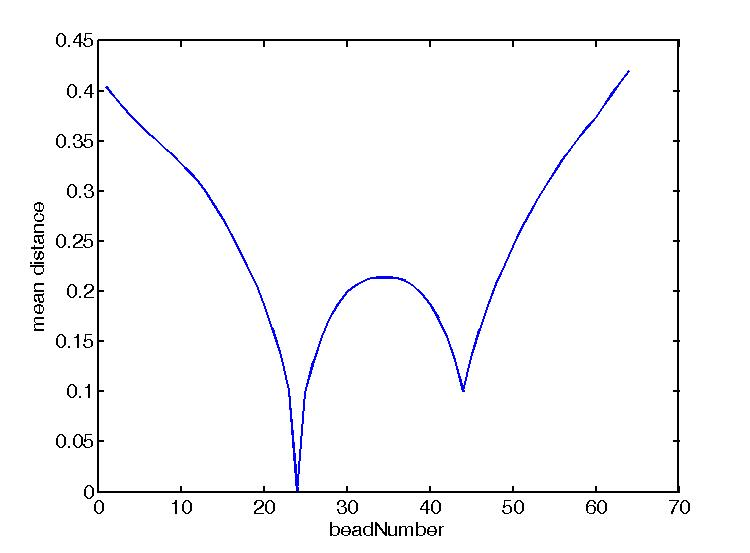
\includegraphics[scale=0.3]{crossectionAtRow24DistanceMatrix64BeadsConnect24And44}
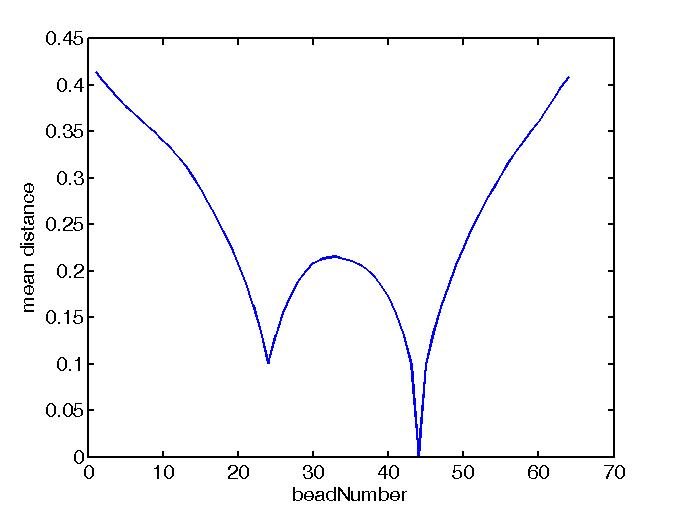
\includegraphics[scale=0.32]{crossectionAtRow44DistanceMatrix64BeadsConnect24And44}
\caption{\scriptsize{The cross section of the mean bead distance matrix presented in Figure \ref{distanceMatrix64BeadsConnect24And44} for bead 24 (left) and bead 44 (right). The height at point 44 (left panel) and point 24 (right panel) is the bond length $b=0.1$ as expected.}}
\label{crossectionAtRow24DistanceMatrix64BeadsConnect24And44}
\end{figure}

\subsubsection{Increasing the encounter distance}
Next we examined whether changing the encounter length in the cross-linked chain can explain the appearance of TADs. The encounter frequency between any two beads of the chain is shown in Figure \ref{encounterFreq64BeadsConnect24And44VaryEncounterLength}. The encounter length varied between half and twice of the connector length (0.1).

\begin{figure}[H]
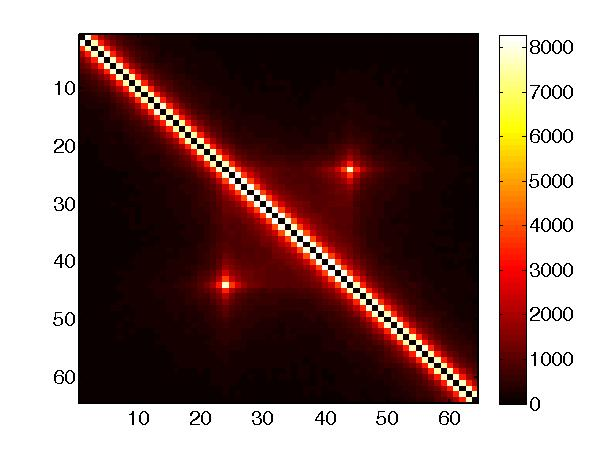
\includegraphics[scale=0.2]{encounterFrequency64BeadsConnect24And44EncounterDist0_05}
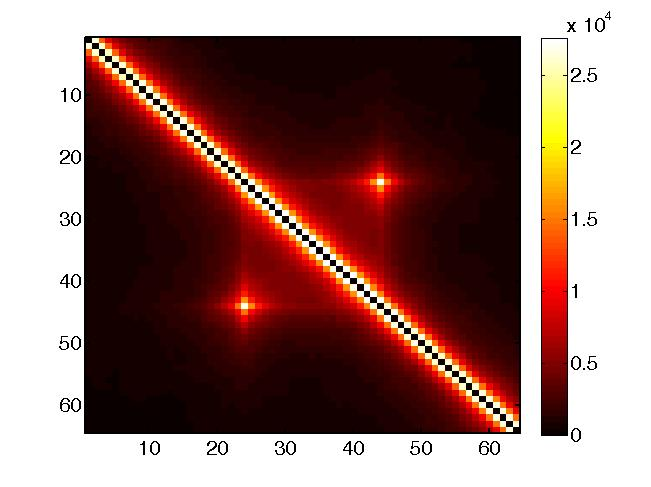
\includegraphics[scale=0.19]{encounterFrequency64BeadsConnect24And44EncounterDist0_1}
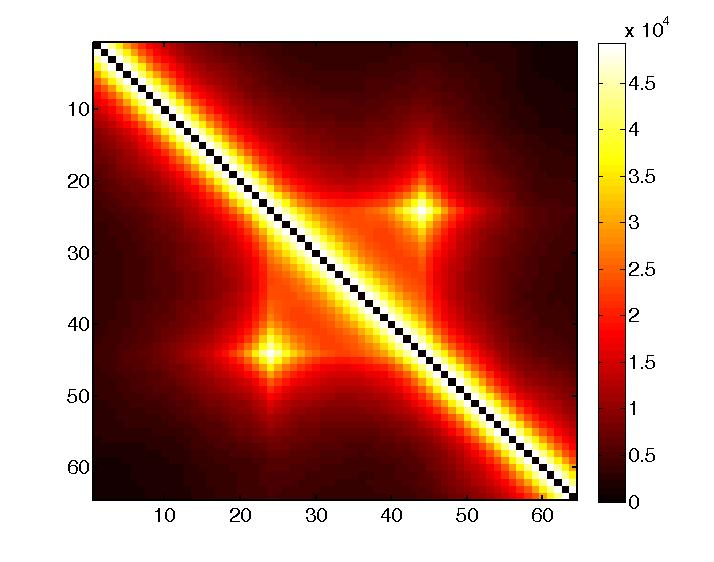
\includegraphics[scale=0.17]{encounterFrequency64BeadsConnect24And44EncounterDist0_2}
\caption{\scriptsize{Encounter frequency matrices of a Rouse polymer with 64 beads with bead 24 and 44 connected by harmonic potential when varying the encounter distance from 0.05 (left), 0.1 (middle), and 0.2 (right). The bond length was set to $b=0.1$, the encounter distance was set to 0.1. Simulation ran over 50,000 steps of $10^{-4}$ seconds. Each pixel represent bead pair $(i,j)$ of the polymer.}}
\label{encounterFreq64BeadsConnect24And44VaryEncounterLength}
\end{figure}

The encounter histogram of bead 24 is displayed in Figure \ref{encounterHistBead24connect24And44EncounterDist0_1}.
\begin{figure}[H]
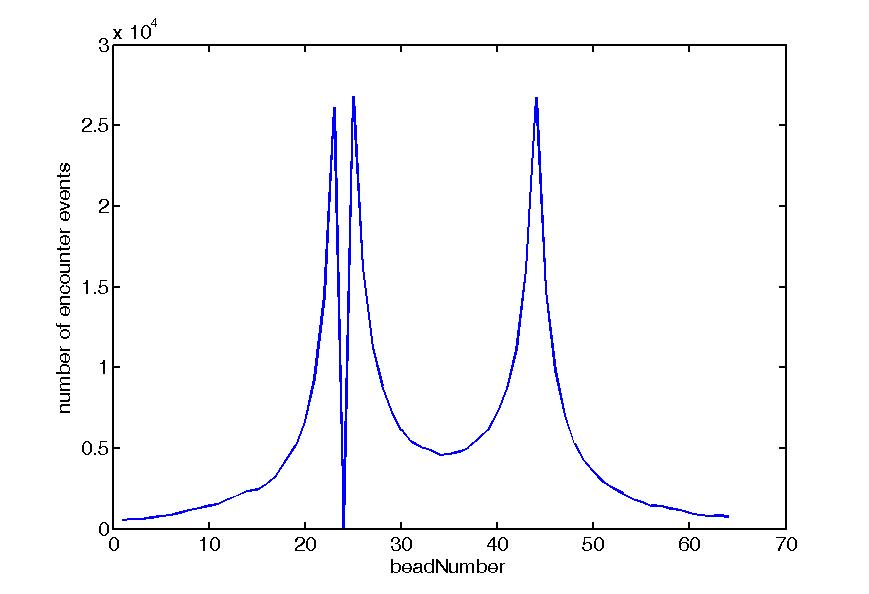
\includegraphics[scale=0.4]{encounterHistBead24connect24And44EncounterDist0_1}
\caption{\scriptsize{the encounter histogram of bead 24 as a function of bead number. The polymer included 64 beads with Kuhn length of 0.1, the encounter distance was set to be 0.1. the self encounters were trivially zeroed out}}
\label{encounterHistBead24connect24And44EncounterDist0_1}
\end{figure}

\subsection{Simulating cross-linked polymer with subsequent cross-link}
To explore the characteristics of the polymer dynamic system with one link, we construct a Rouse polymer with 32 beads, and subsequently link bead $i$ to bead $j$, where $i=1,2,...14$, $j=i+2,i+3,..,30$. The time step was determined to be $\Delta t = 5\times10^{-4}$ sec, over a series of 3500 steps. 

The eigenvalues and eigenvectors of the \textit{mean} bead distance matrix were calculated.
Eigenvalues were sorted in ascending order. In all simulation eigenvalues were negative except one, which took on a high positive value in relation to the other eigenvalues. 

A characteristic pattern can be seen in Figure \ref{eigenValuesOfTheDistanceMatrix}

\begin{figure}[H]
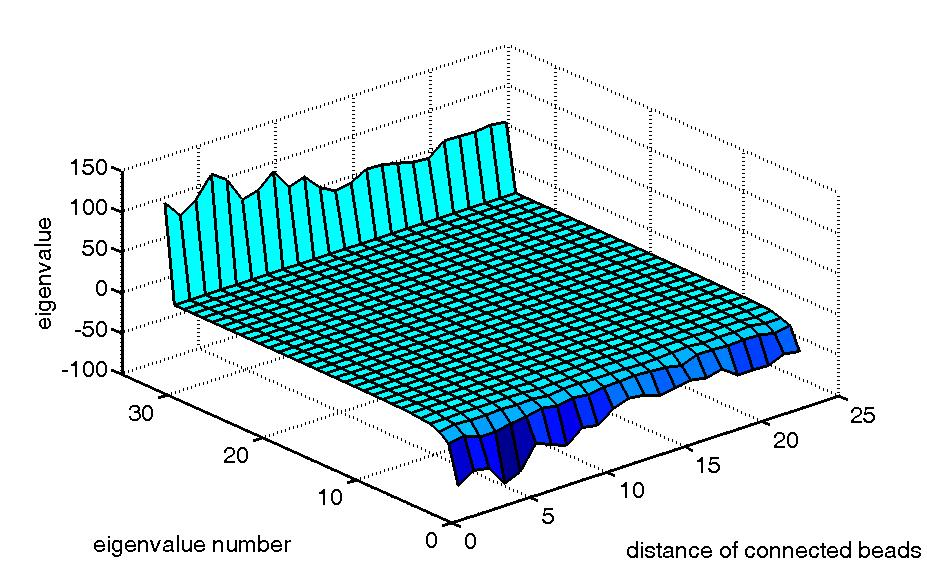
\includegraphics[scale=0.2]{eigenValuesofTheDistanceMatrix32BeadsBead8IsConnected}
\caption{\scriptsize{a surface representing the sorted eigenvalues}}
\label{eigenValuesOfTheDistanceMatrix}
\end{figure}

\subsection{Simulation of variable loop number}
\subsection{One TAD}
To examine the effect of increasing the number of stable loops on the encounter probability, a chain of 32 beads was constructed. The number of stable loops varied from 0 to 16. the bond length $b=0.1$, the encounter distance was set to $b/2=0.05$, the time step was set to prevent simulation blow ups by the formula above, $\Delta t=8.3\times10^{-4}$. For each number of loops, random pairs of beads were chosen to be connected. 
\begin{figure}[H]
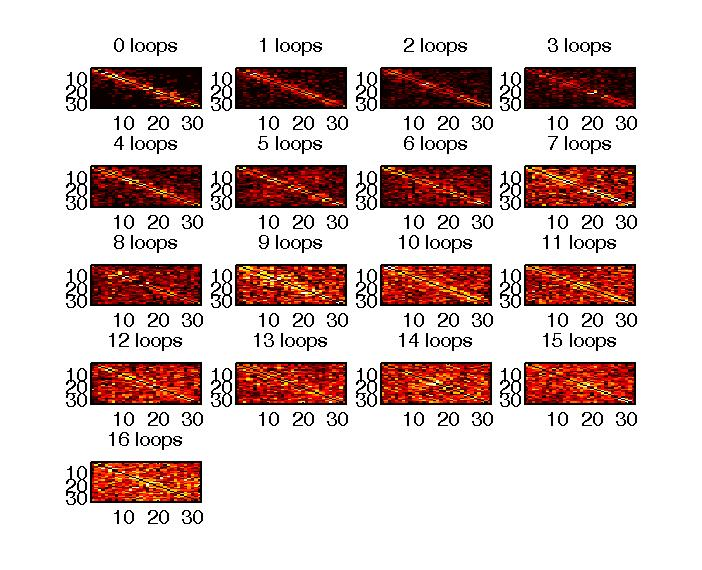
\includegraphics[scale=0.4]{stableLoopModelVariableLoopNumber32Beads}
\caption{\scriptsize{The encounter histogram of a chain of 32 beads. When the number of loops varies from 0 to 16 an area resembling a TAD emerges}}
\label{stableLoopModelVariableLoopNumber32Beads}
\end{figure}

for each choice of loop number, we fit a curve to the encounter probability as a function of distance.
\begin{figure}[H]
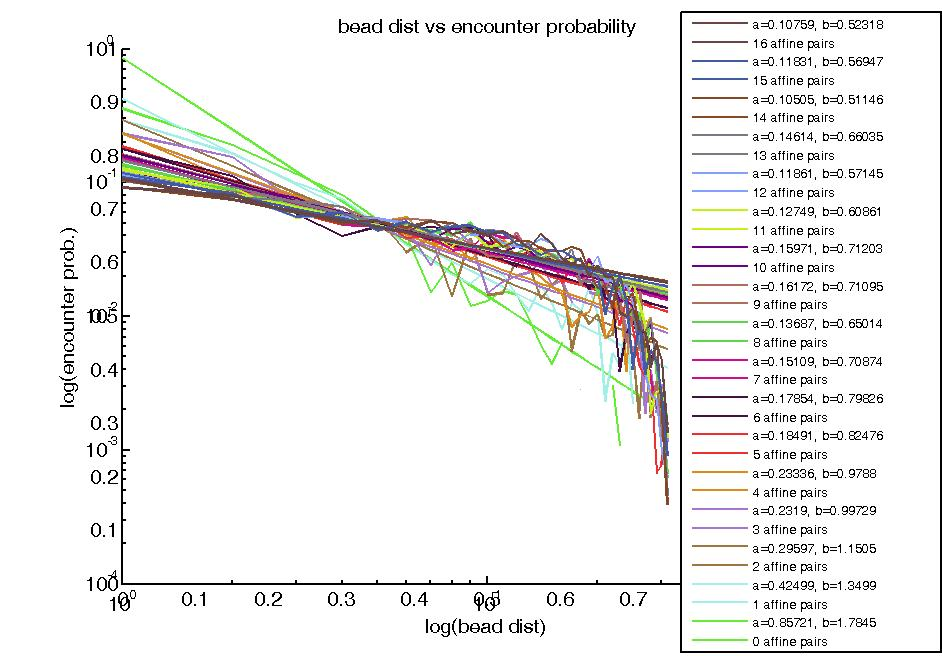
\includegraphics[scale=0.3]{logBeadDistanceVsEncounterProbabilityVariableLoops32Beads}
\label{logBeadDistanceVsEncounterProbabilityVariableLoops32Bead}
\end{figure}

The fitted exponent values are decreasing roughly quadratically. 
\begin{figure}[H]
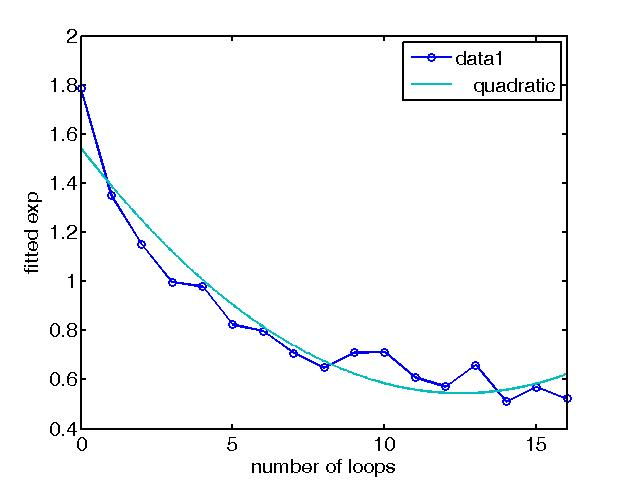
\includegraphics[scale=0.3]{changeOfExponentAsAfunctionOfLoopsStableLoopModelVariableLoops32Beads}
\label{changeOfExponentAsAfunctionOfLoopsStableLoopModelVariableLoops32Beads}
\end{figure}
	
\subsubsection{One TAD with 'tail'}
In this simulation we test the affect of the increase in the number of stable loops on the bead encounter probability. An ensemble of chains comprised of 64 beads were simulated to $1.2$ times the relaxation time of the first Rouse mode, resulting in about $16,000$ steps for each chain. For each loop number 300 simulation were carried out. The bond length was set to be $b=0.1$, the encounter distance $\epsilon=b/2$, time step was set to be $\delta t=10^{-4}$. Stable loops were defined between bead $1$ and $32$ which we expect to resemble a TAD. At each simulation round we increase the number of loops $L$ by choosing at random $2L$ bead indexes of bead to be connected, $L$ is varied from 0 to 15. the encounter histogram shows an increasing encounter pattern in the region the loops are defined in (see Figure \ref{stableLoopModelVariableLoopNumber64Beads})
 
\begin{figure}[H]
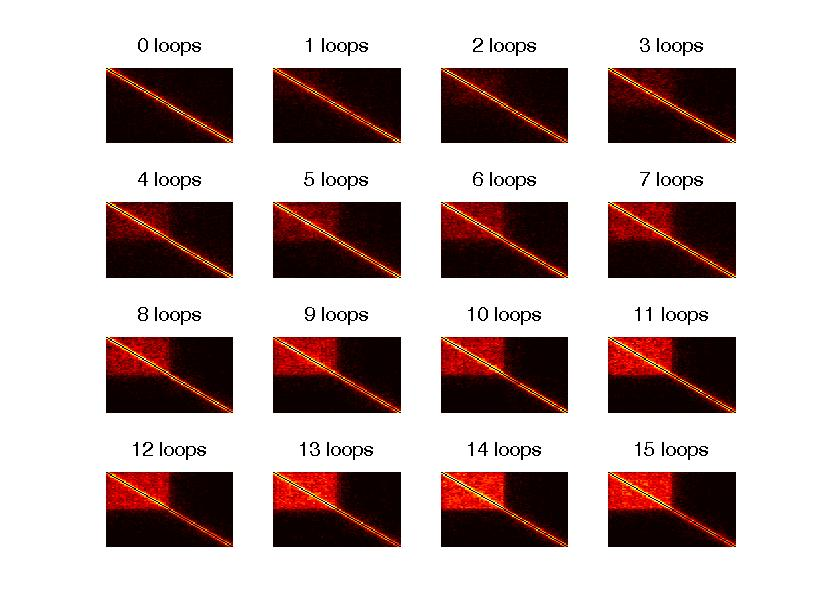
\includegraphics[scale=0.3]{stableLoopModelVariableLoopNumber64Beads}
\caption{\scriptsize{The affect of increasing the stable loops in a polymer of 64 beads. Loops were created at random between beads located in the first half of the polymer. Increasing the number of loops from 0 to 15 reveals a region resembling a TAD as seen in the data}}
\label{stableLoopModelVariableLoopNumber64Beads}
\end{figure} 
 
 The encounter probabilities for the chains when increasing the loops from 0 to 15, can be seen in Figure \ref{logBeadDistanceVsEncounterProbabilityVariableLoops64Beads}
For each encounter probability curve we fit a function of the form $ad^{-b}$. The change in the exponent $b$ as a function of the number of loops is seen in Figure \ref{changeOfExponentAsAfunctionOfLoopsStableLoopModelVariableLoops64Beads}

\begin{figure}[H]
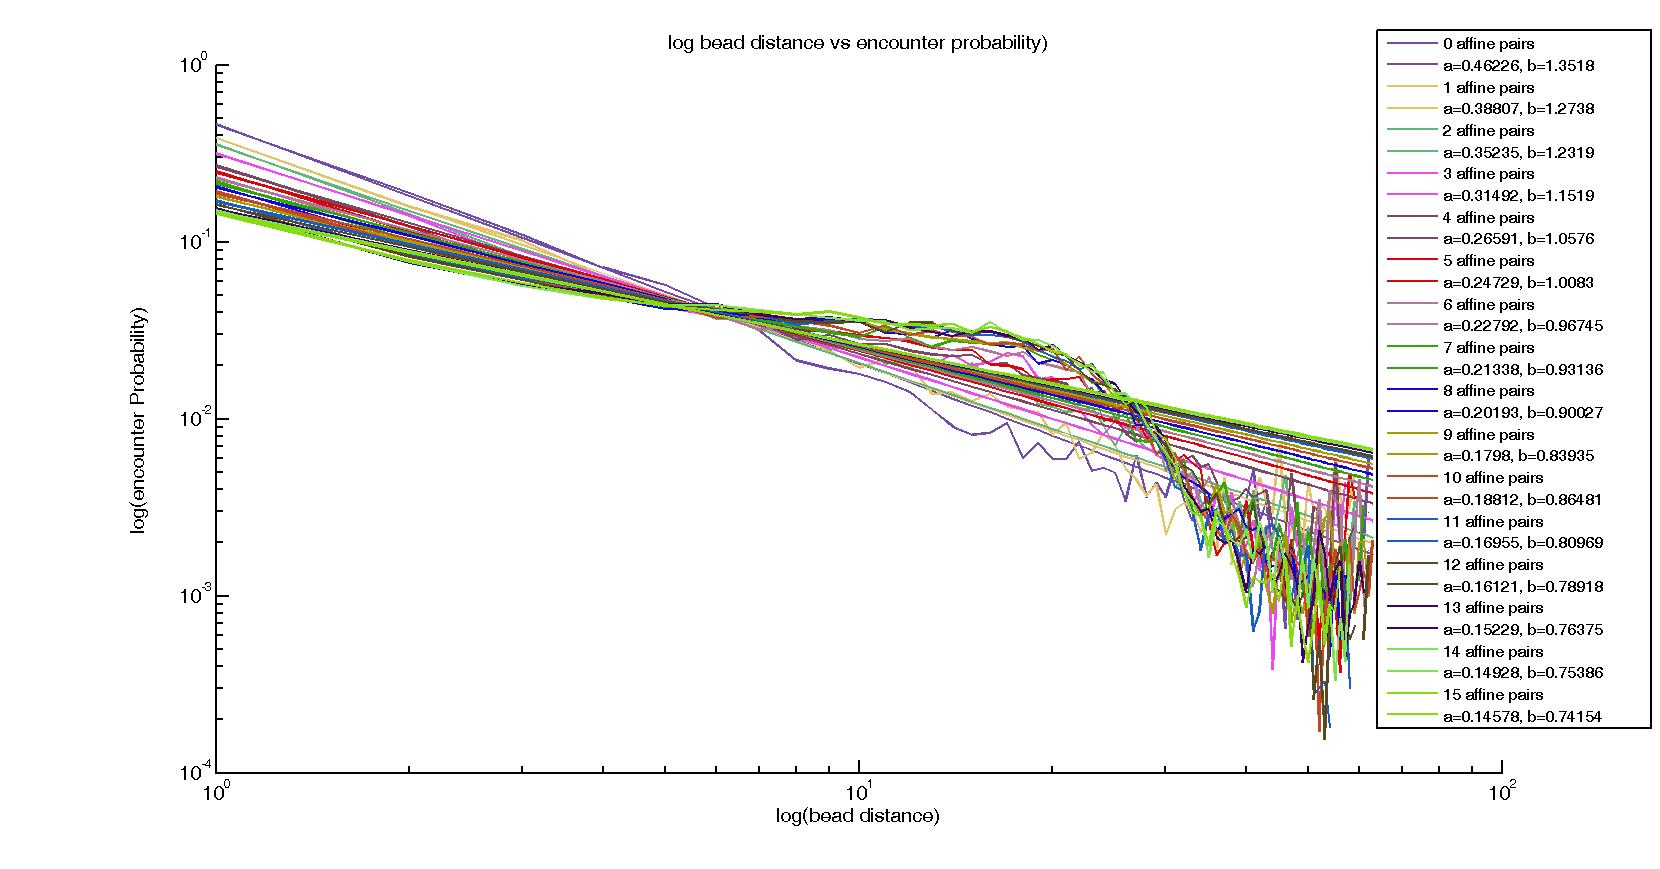
\includegraphics[scale=0.2]{logBeadDistanceVsEncounterProbabilityVariableLoops64Beads}
\caption{\scriptsize{Encounter probability vs bead distance for the 16 models representing variable stable loops number if the first half of the chain of 64 beads (top)}}
\label{logBeadDistanceVsEncounterProbabilityVariableLoops64Beads}
\end{figure}

\begin{figure}[H]
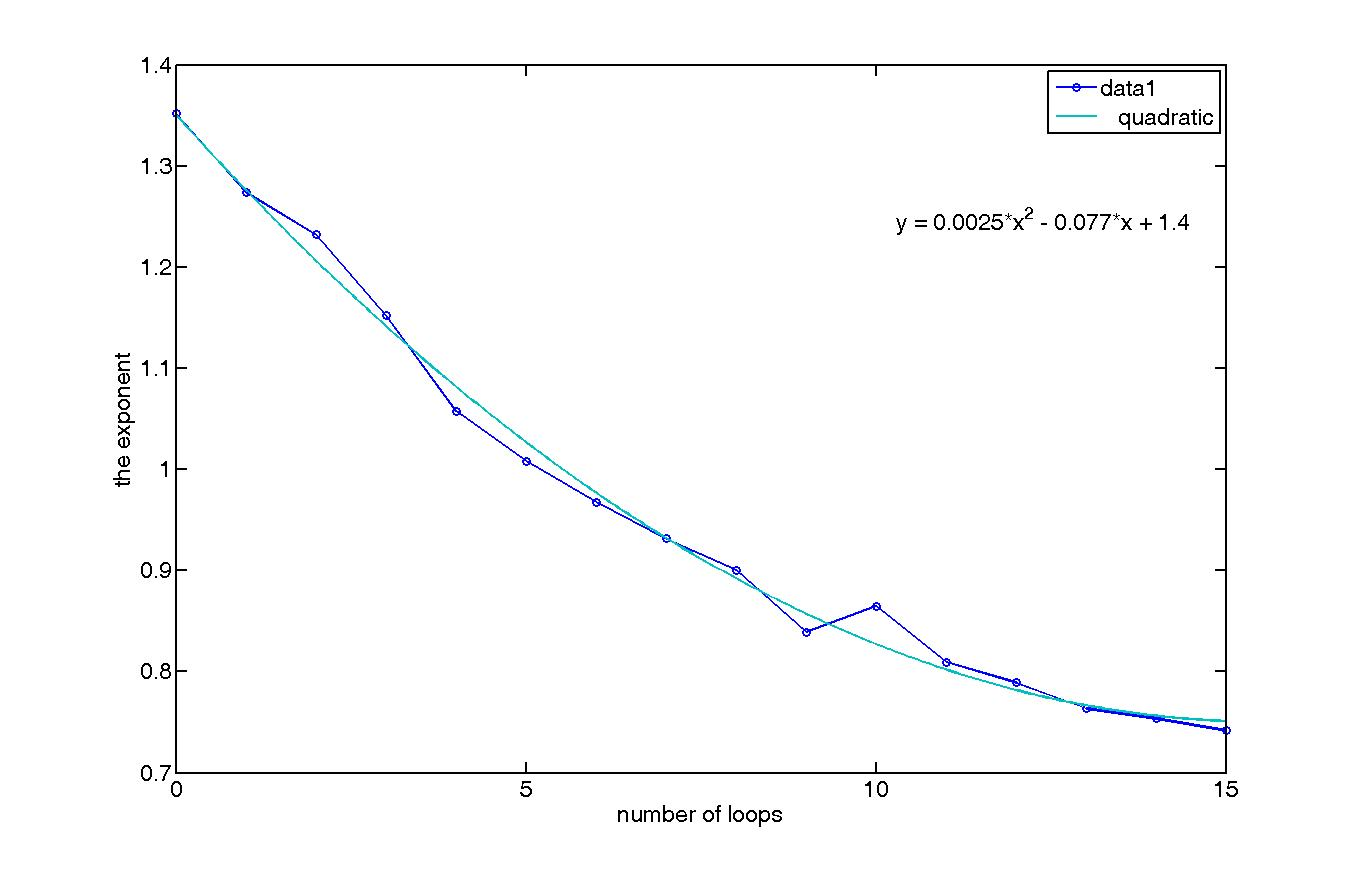
\includegraphics[scale=0.15]{changeOfExponentAsAfunctionOfLoopsStableLoopModelVariableLoops64Beads}
\caption{\scriptsize{The change in the value of the fitted exponent to the encounter probability curves of models with increasing number of stable loops. The decrease in the values of $b$ quadratic as can be seen by the cyan line fitted to the data.}}
\label{changeOfExponentAsAfunctionOfLoopsStableLoopModelVariableLoops64Beads}
\end{figure}
\subsubsection{Two TADs}
 

\subsection{Simulating dynamic loops model}
It can be assumed that stiff fixed loops in the chromatin are not always stable, but can open and close transiently. We turn to examine whether a model with loops that can be formed, held fixed, for some period, and be released, can explain the appearance of the TADS. The rational behind is that the variability of cells used in the experiments some in different states, i,e. are found with different initial chromatin loops. When these cells are fixed and the chromatin is cross-linked, the cross-links that will form will depend on the proximity of the beads conditional on the loops present at the moment the experiment began. 


A polymer with 128 beads was simulated. We define two region with high affinity of their member beads to a specific point in them. These regions can be considered as the TADs. Each region is of size $25$ beads. The first region is defined to be from bead 1 to 25, the second from bead $77$ to $102$. 

To simulate the state of experiment initiation, we define two beads in each TAD, which have high probability to be found together, and run simulations until steady state. Only one pair from each TAD was examined in each simulation, which we vary from simulation to simulation. At the end of each simulation we retrieve the encounters frequency for all the beads. 

Beads that come in close proximity to one another, are considered attached, and can be released and some rate $k_{off}$. The attachment distance was defined as half of the connector length between adjacent beads. 

\begin{figure}[H]
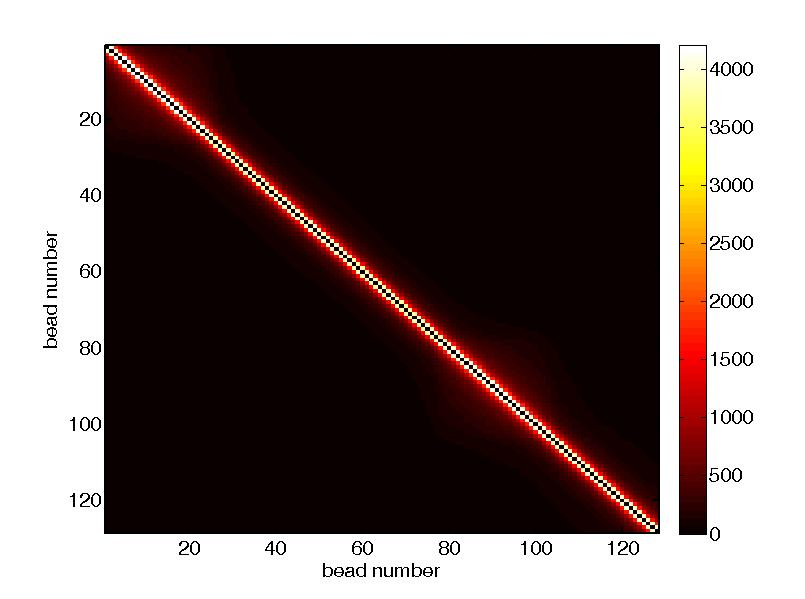
\includegraphics[scale=0.2]{encounterFrequency128beadsWithTadTransientModel}
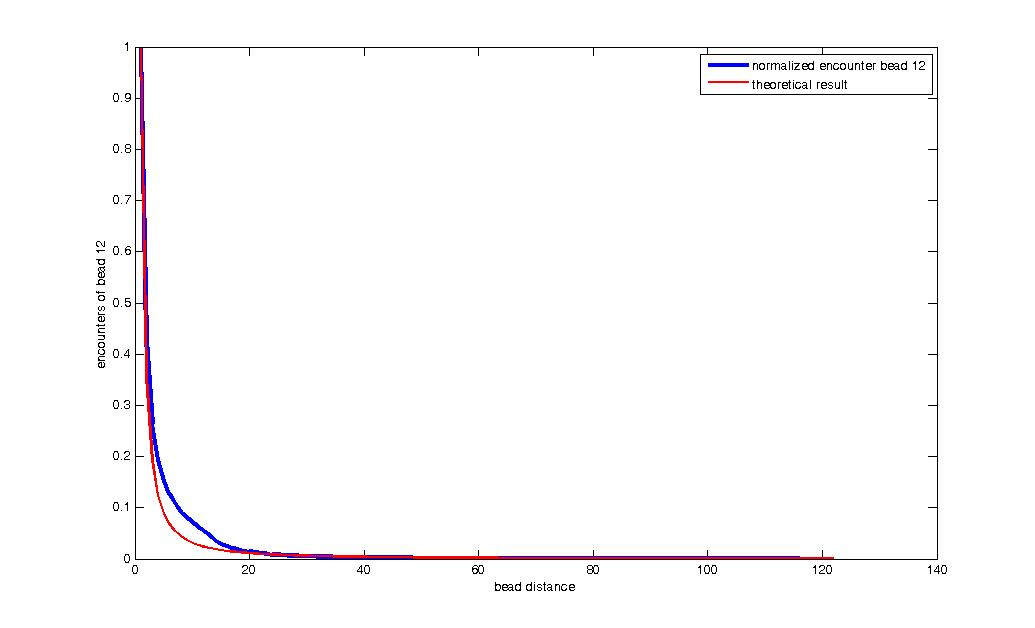
\includegraphics[scale=0.2]{encounterCrossectionBead12TransientLoopModelwithTheoreticalCurve}
\caption{\scriptsize{The mean encounter matrix for the transient loop model. the chain included 128 beads, with connector length of 0.1. Two regions were defined as the TADs: Bead 1 to bead 25, and bead 77 to 102. at each simulation, a pair of beads from each region were considered as having some affinity to one another. The model was simulated for each choice of affine pair until steady-state, 30000 steps. The mean encounter of all simulation in presented.}} 
\end{figure}

For beads that are not affine to any other, like the beads 26 to 77, the encounter frequency retrieved matches the theoretical result. 

\subsection{Simulating the 3C experiment}
Next simulated  the conditions of the 3C experiment to examine whether we can retrieve the TADs. The simplified version of the experiment is simulated, i.e. we  take a Rouse chain comprised of 128 beads, we simulate the chain until steady-state, and we 'freeze' the picture. We then find all beads located within a distance $\epsilon$ from one another. At the end of the simulation we sum over all realizations and call it the encounter matrix. 

The main difference between simulating a Rouse chain many times and performing this experiment is that in the the former, we simulate until steady state and from steady state onward we recored the encounter frequency at each step. The result is the encounter matrix of a \textit{single} chain evolving in time. In this experiment, we simulate different chains, with different initial condition, and the end result is the sum of encounters of \textit{different} chains. 

The results show a strong deviation from the theoretical result. The encounter frequency of each bead decayed much slower than $N^{-1.5}$. Although this result can not explain the appearance of two different regions which have lower interactions among them, it can be form the basis for the understanding of the behavior of encounters in each one of the TADs. In later experiments we will try to change the architecture of the chain, making it heterogenic, by placing stiff boundaries between TADs. 

\begin{figure}[H]
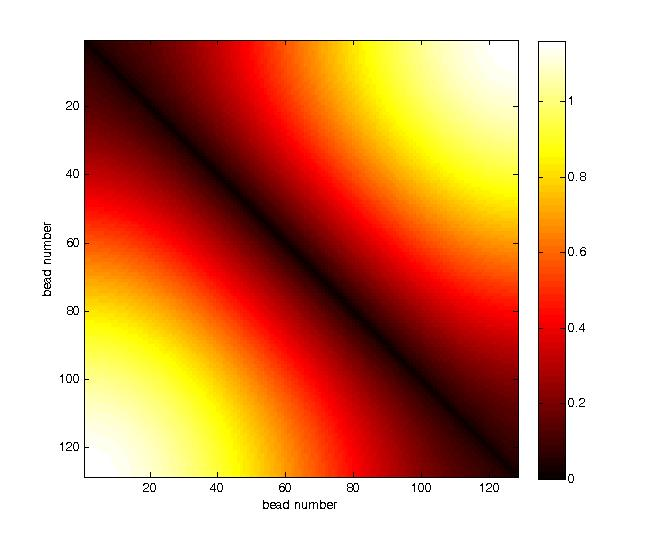
\includegraphics[scale=0.2]{encounterMatrix3cExperiment}
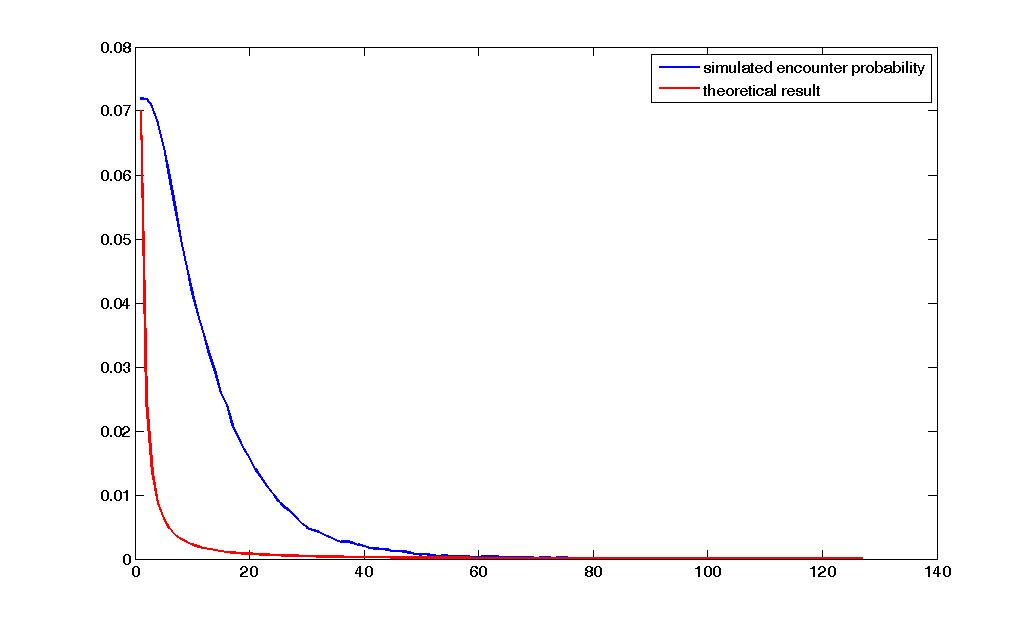
\includegraphics[scale=0.2]{encounterProbabilityBead1OfThe3cSimulation128Beads}
\caption{The encounter matrix and encounter probability profile for the simulated 3C experiment. The encounter matrix (left) still shows a decaying pattern of encounter.}
\end{figure}

\subsection{Simulating dense regions}
To verify that regions in the boundaries of the TADs are responsible for the interaction maps viewed in the article by Nora et al. We simulate a chain comprised of 120 beads. We cross-link a group of adjacent beads at two locations along the chain, the group 30-40 and the group 80-90. 3500 simulation steps are performed with a step size of $\Delta t = 5\dot10^{-4}$ sec. 

\subsection{Simulating TAD D and E with cross-links corresponding to the peaks of 5C data}
We next wanted to verify whether using a Rouse polymer and connecting beads for which the peaks of the experimental data, would allow us to reproduce the TADs. 

A polymer with 307 beads was created, corresponding to the TAD D (107 beads) and E (200 beads). The cross-links were made at the mid point of bead numbers displayed in Table \ref{nonNeighborBeadEncounterTable}. Thirty simulations were performed and their average distance matrix after relaxation time is presented in Figure \ref{meanEncounterMatrixOfSimulatingTADEandDWithLoops}. As can be seen the location of the cross-links create 'hot spots' in the mean distance matrix. In comparison to Figure \ref{TADsOfTheXChromosome}, we see that there is little resemblance. Thus concluding that creating cross-links according to the encounter matrix, is not sufficient to reproduce the TADs.

\begin{figure}[H]
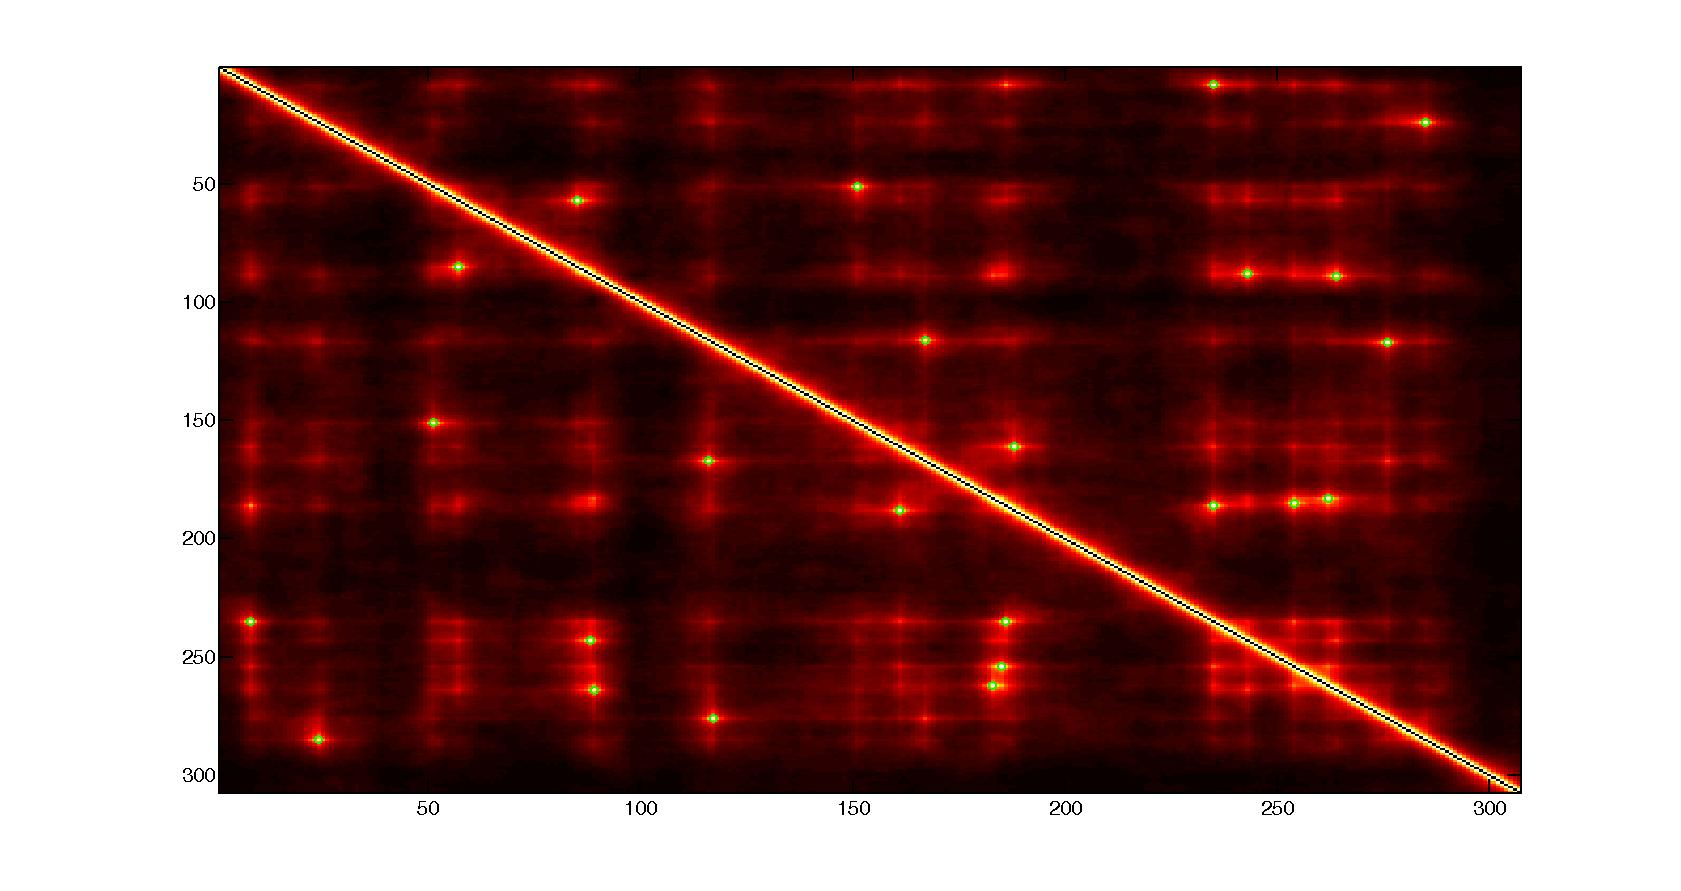
\includegraphics[scale=0.2]{meanEncounterMatrixOfSimulatingTADEandDWithLoops}
\caption{\scriptsize{The mean of 30 simulation of the polymer with 307 beads, connected corresponding to the peaks of the encounter data (Luca et al). The small green circles represent locations of connected bead pairs. These circles overlap with peaks of the simulated encounter matrix. It is evident that the TAD structure was not reproduced with this approach. The x and y axes  represent bead numbers. Each pixel represents the encounter number of bead $i$ and $j$}}
\label{meanEncounterMatrixOfSimulatingTADEandDWithLoops}
\end{figure}

\subsection{Simulating the conditional encounter probability}
In these simulation we empirically find what is the probability that a bead $A$ meets a bead $B$ before it meets bead $C$. For this end, a chain of 32 beads was constructed. Each simulation contained 5 times the relaxation steps, in a total of 150 simulations for each choice of bead $n$. We vary bead $B$, from 2 to 31.$A$ was set to 1, $C$ was set to 32.

\begin{figure}[H]
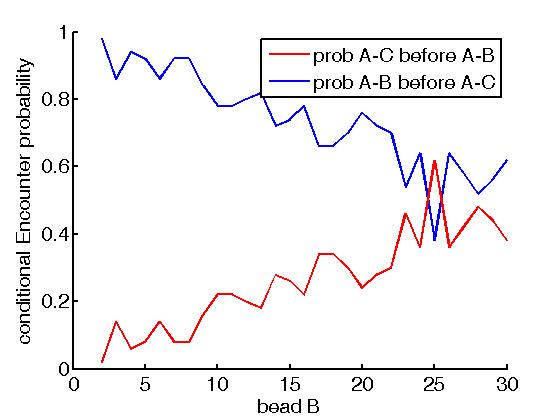
\includegraphics[scale=0.3]{conditionalEncounterProb32BeadsVaryBead2From2To31}
\caption{\scriptsize{The conditional probability that bead 1 will meet bead 2 to 32}}
\label{conditionalEncounterProb32BeadsVaryBead2From2To31}
\end{figure}

\subsection{simulating the effect of increasing the encounter distance}
In a chain of 32 beads, we increase the encounter distance and examine the difference in the encounter probability. 
The bond length was set to $b=0.1$, the encounter distance was set to increase from $b/4$ to $2b$ with an increment of 0.01, a total of 18 simulation rounds. For each choice of encounter distance 50 simulation were preformed. simulations were ran to 5 times the relaxation time of the first Rouse mode. 



\section{Review Of Literature}

\subsection{From Nora et.al 2012 \cite{nora2012spatial}}
\begin{itemize}
\item The X inactivation center (Xic) orchestrate the initiation of the X chromosome inactivation by controlling the expression of non-protein-coding Xist transcript. 
\item 5C techniques were  used to analyze the \textit{spatial} organization of the region including the Xist. The region analyzed  is 4.5 Mb in size. 
\item 200 kb to 1 Mb regions were discovered and named TAD.
\item TADs remain consistent between male and female Embryonic stem cells (ESC) and betwee different cell lines.
\item TADs remain persistent before and after cell differentiation and before and after X inactivation. Internal TAD connections remain high even after X inactivation. However, the intra-TAD connection are lower than those of the same TAD on the active X.
\item on the inactive X, the long range interaction($>50kb$) inside the TAD are lost. 
\item disrupting the regions between TADs caused an ectopic chromosomal contacts 
\item 5C-Forward and 5C-Reverse oligonucleotides were designed to conduct test on undifferentiated mouse embryonic stem cells (ESCs)
\item it was found that long range contacts (>50kb) happen within a series of discrete genomic blocks , roughly 0.2-1 Mb in size 
\item The chromosomal domains are self-associating. 
\item FISH experiment on 3D chromosomal conformation were conducted to verify the results.
\item in the FISH, the distance between probes lying in the same 5C domain were significantly shorter than of probes lying in different domains. 
\item a strong correlation was found between 5C count and 3D distance. 
\item bacterial artificial chromosome probes showed in experiments that large DNA segments belonging to the same 5C domain co-localize much more than DNA segment on adjacent domains \textit{throughout cell cycle}. 
\item a correlation was shown between the existence of H3K27me and the TADs. However, for a mouse with a knockout of these proteins, a significant change was \textit{not} observed in the composition and size of the TADs.
\item it was shown that H3K27me - an antibody signifying the presence of Histone 3- is not related to the folding of the genomic regions into TADs. 
\item when the boundary between TAD E and D (which include the Xist and Tsix), ectopic folding of TAD E was observed. It was assumed that boundary elements have an influence on the conformation of the TADs. 
\item after removing boundary elements between TADs, the TADs did not merge completely, hence concluded that there are other, intra-TADs element that control conformation.
\item TAD did not change during cell differentiation (from embryonic stem cell to neuronal progenitor and embryonic fibroblast), but the \textit{internal} connections inside each TAD did change.
\item for the TADs that did change, some have become \href{http://www.nature.com/nature/journal/v453/n7197/full/nature06947.html}{Lamina Associated Domains} (LADs) 
\item the transcription dynamics showed positive correlation for TADs for which the promoter of the genes was located inside the TAD. 
\item the correlation between gene expression of genes in the same TAD did not depend on the distance between genes in the TAD. 
\end{itemize}

\subsection{From Dekker et al 2013 \cite{dekker2013exploring}}

% Bibliography  
\bibliographystyle{plain}
\bibliography{PolymerChainDynamicsSummaryOfFindingsBibliography} % the bibliography.bib
\end{document}